\chapter{Experimental Setup}
\label{chap:exper_setup}
\epigraph{If it disagrees with experiment, it’s wrong. In that simple statement is the key to science. It doesn’t make any difference how beautiful your guess is, it doesn’t matter how smart you are who made the guess, or what his name is \ldots  If it disagrees with experiment, it’s wrong. That’s all there is to it.}{\textit{Richard Phillips Feynman}}
In this chapter, we describe the experimental setup used to collect the data used for the searches. We first describe the collider which smashes protons together. Then we describe the detector used to collect the data from those proton-proton collisions.
\section{The Large Hadron Collider}
\label{sec:LHC}

The Large Hadron Collider (LHC)~\cite{lhcmachine} is a powerful proton-proton synchrotron. It was built and is operated at the European Center for Nuclear Research (CERN) and is situated about 100 m underground close to Geneva, Switzerland. It has a circumference of 26.7 km and uses a tunnel previously built for LEP (Large Electron Positron Collider). Being a particle-particle collider, it consists of two rings with counterrotating beams which are steered using magnets and accelerated using radiofrequency resonating cavities. These beams are made to intersect at four collision points around the LHC ring, at one of which rests the CMS detector. Besides proton-proton collisions the LHC can also collide heavy ions (lead-lead collisions) or heavy ions with protons (lead-proton collisions). Since starting operation in September 2008, the LHC has been the world's most powerful apparatus and will probably remain so in the forseeable future. The following section describes proton-proton collisions at the LHC as the data used in the subsequent physics analysis corresponds to events from these collisions.

The injector chain that supplies protons to the LHC consists of four CERN accelerators that actually predate the LHC: Linac 2, PSB (Proton Synchroton Booster), PS (Proton Synchotron) and SPS (Super Proton Synchotron). This is illustrated in figure~\ref{fig:cern_acc_comp}. The proton source is simply a tank of hydrogen gas. The hydrogen atoms are ionized to yield protons which are then fed in to the Linac 2, a linear accelerator. This accelerates the protons to an energy of about 50 MeV which are then fed into a series of circular accelerators, starting with the PSB which accelerates the protons to 1.4 GeV. The PS then accelerates them to 25 GeV, and they are then sent to the SPS which accelerates them to 450 GeV before being finally fed into the LHC beampipe. Inside the LHC the protons are accelerated by sixteen radiofrequency cavities which are made to oscillate at 400 MHz and the proton beam is sorted into discrete packet called ``bunches''. The beam is steered by 1232 Niobium-Titanium superconducting dipole magnets and collimated using quadrupole magnets. This magnet system is kept at a temperature below 2 K, using a pressurised bath of superfluid helium at about 0.13 MPa, and operates at fields above 8T. The LHC has three sophisticated vacuum systems: the insulation vacuum for cryomagnets, the insulation vacuum for helium distribution, and the beam vacuum.

\begin{figure*}
\begin{center}
\includegraphics[width=0.8\textwidth,keepaspectratio]{plots_and_figures/chapter3/cern_acc_complex.png}
\caption{Cern Accelerator Complex ~\cite{acc_complex}}
\label{fig:cern_acc_comp}
\end{center}
\end{figure*}


It takes about 4 minutes and 20 seconds to fill up each of the LHC rings wih protons, and about 20 minutes for the proton beam to reach its current peak energy of 6.5 TeV. At this point, each LHC beam contains 2808 bunches with $1.5 \times 10^{11}$ protons per bunch, colliding at a center of mass energy (COM) of 13 TeV. It is anticipated for the COM energy to increase to 14 TeV in 2018. Looking for physics beyond the standard model by colliding protons at such high energies is one of the primary aims of the LHC.

Another important parameter for a collider like the LHC is the instantaneous luminosity (referred to as just luminosity in the following), $\mathscr{L}$. The number of events ($N$) generated per second for some processes is given by:

\begin{equation}
  \frac{dN}{dt}=\sigma\mathscr{L}
\end{equation}


where $\sigma$ is the cross-section of the processes. The luminosity of the LHC can be also expressed in terms of only beam parameters as:

\begin{equation}
  \mathscr{L}=\frac{N_{b}^2 n_{b} f_{rev} \gamma_{r}}{4 \pi \epsilon_{n}\beta^{*}} F
\end{equation}

where $N_{b}$ is number of protons in a bunch, $n_{b}$ is number of bunches per beam, $f_{rev}$ is the revolution frequency, $\gamma_{r}$ the relativistic gamma factor, $\epsilon_{n}$ the transverse beam emittance, $\beta^{*}$ the beta function at the collision point, and F is a reduction factor coming from the fact that the beams cross at an angle.


This luminosity intergrated over time represents the total number of events collected per unit cross section and is called the integrated luminosity ($L$). The LHC has already reached its nominal design luminosity of $10^{34} cm^{-2}s^{-1}$, and it delivered data amounting to a more than $36\,fb^{-1}$, only in 2016. Figure~\ref{fig:cms_int_lumi} shows the amount of data delivered by the LHC overlaid with the subset collected by the CMS detector in 2015 and 2016. The data analysed in the searches described in this thesis were collected by the CMS detector\,(section ~\ref{sec:CMS}) in 2016 during proton-proton collisions delivered by the LHC, and correspond to an integrated luminosity of $35.9\,fb^{-1}$.


\begin{figure*}
\begin{center}
  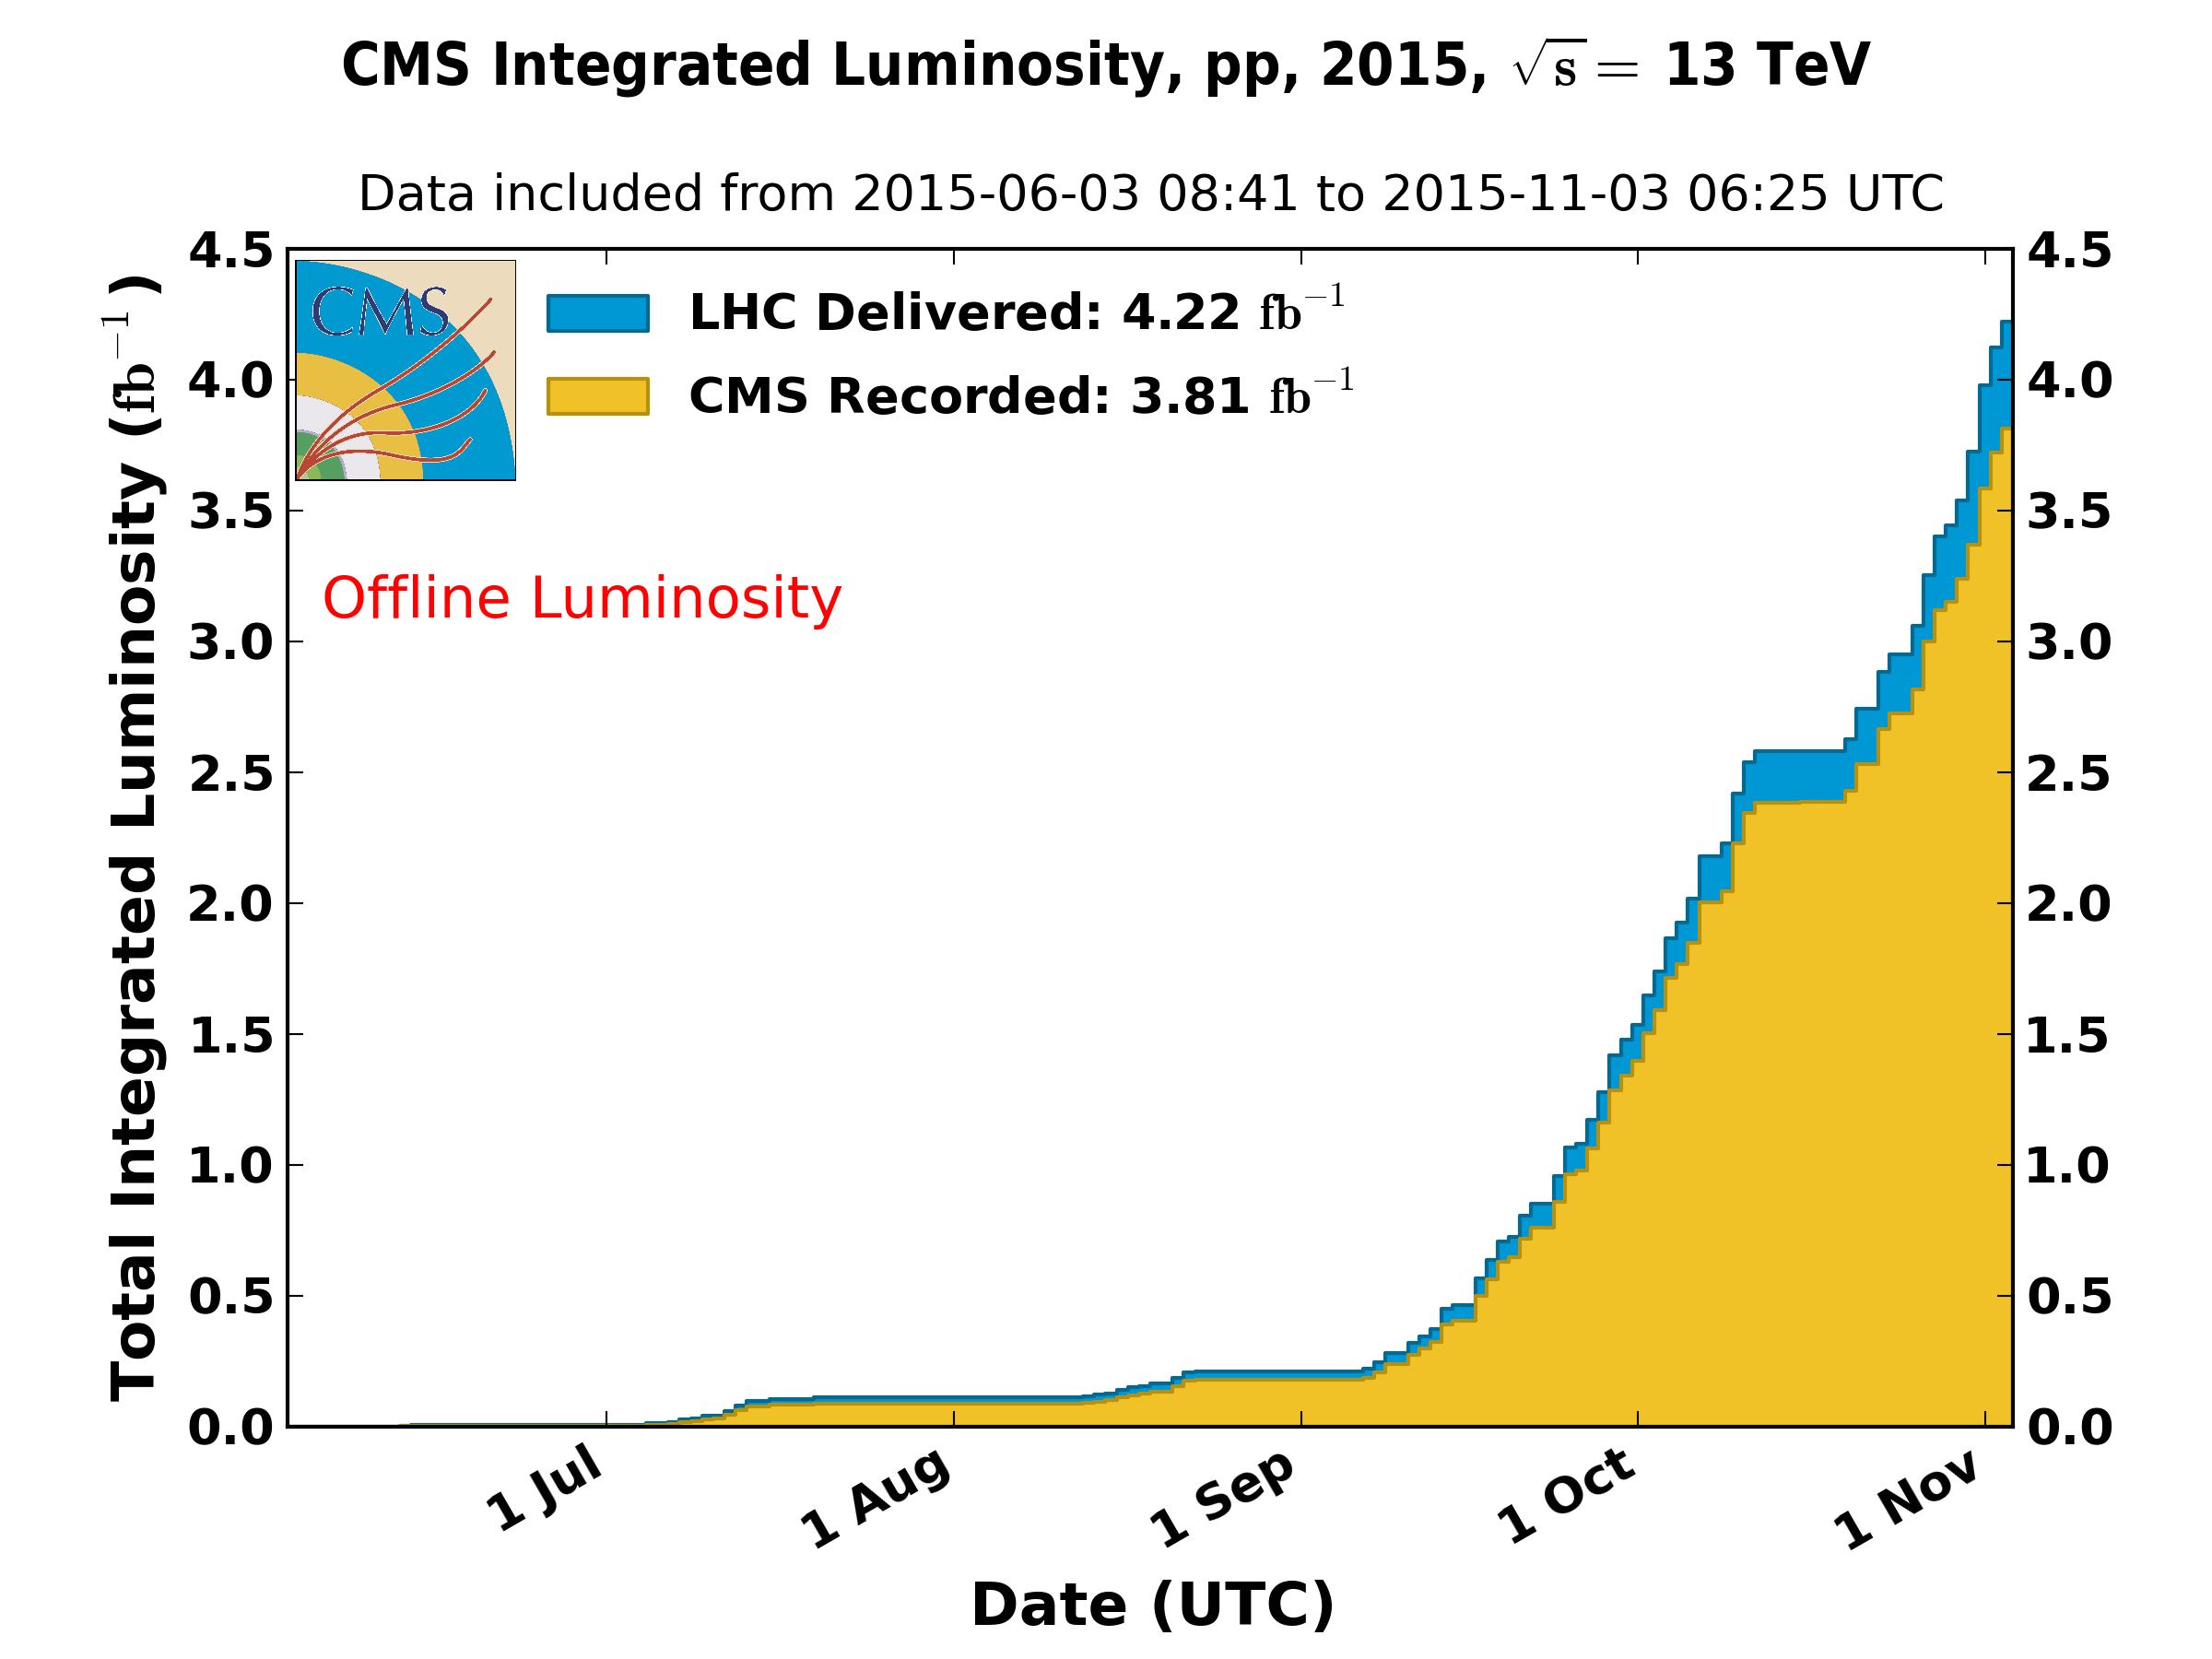
\includegraphics[width=0.4\textwidth,keepaspectratio]{plots_and_figures/chapter3/int_lumi_per_day_cumulative_pp_2015.png}
  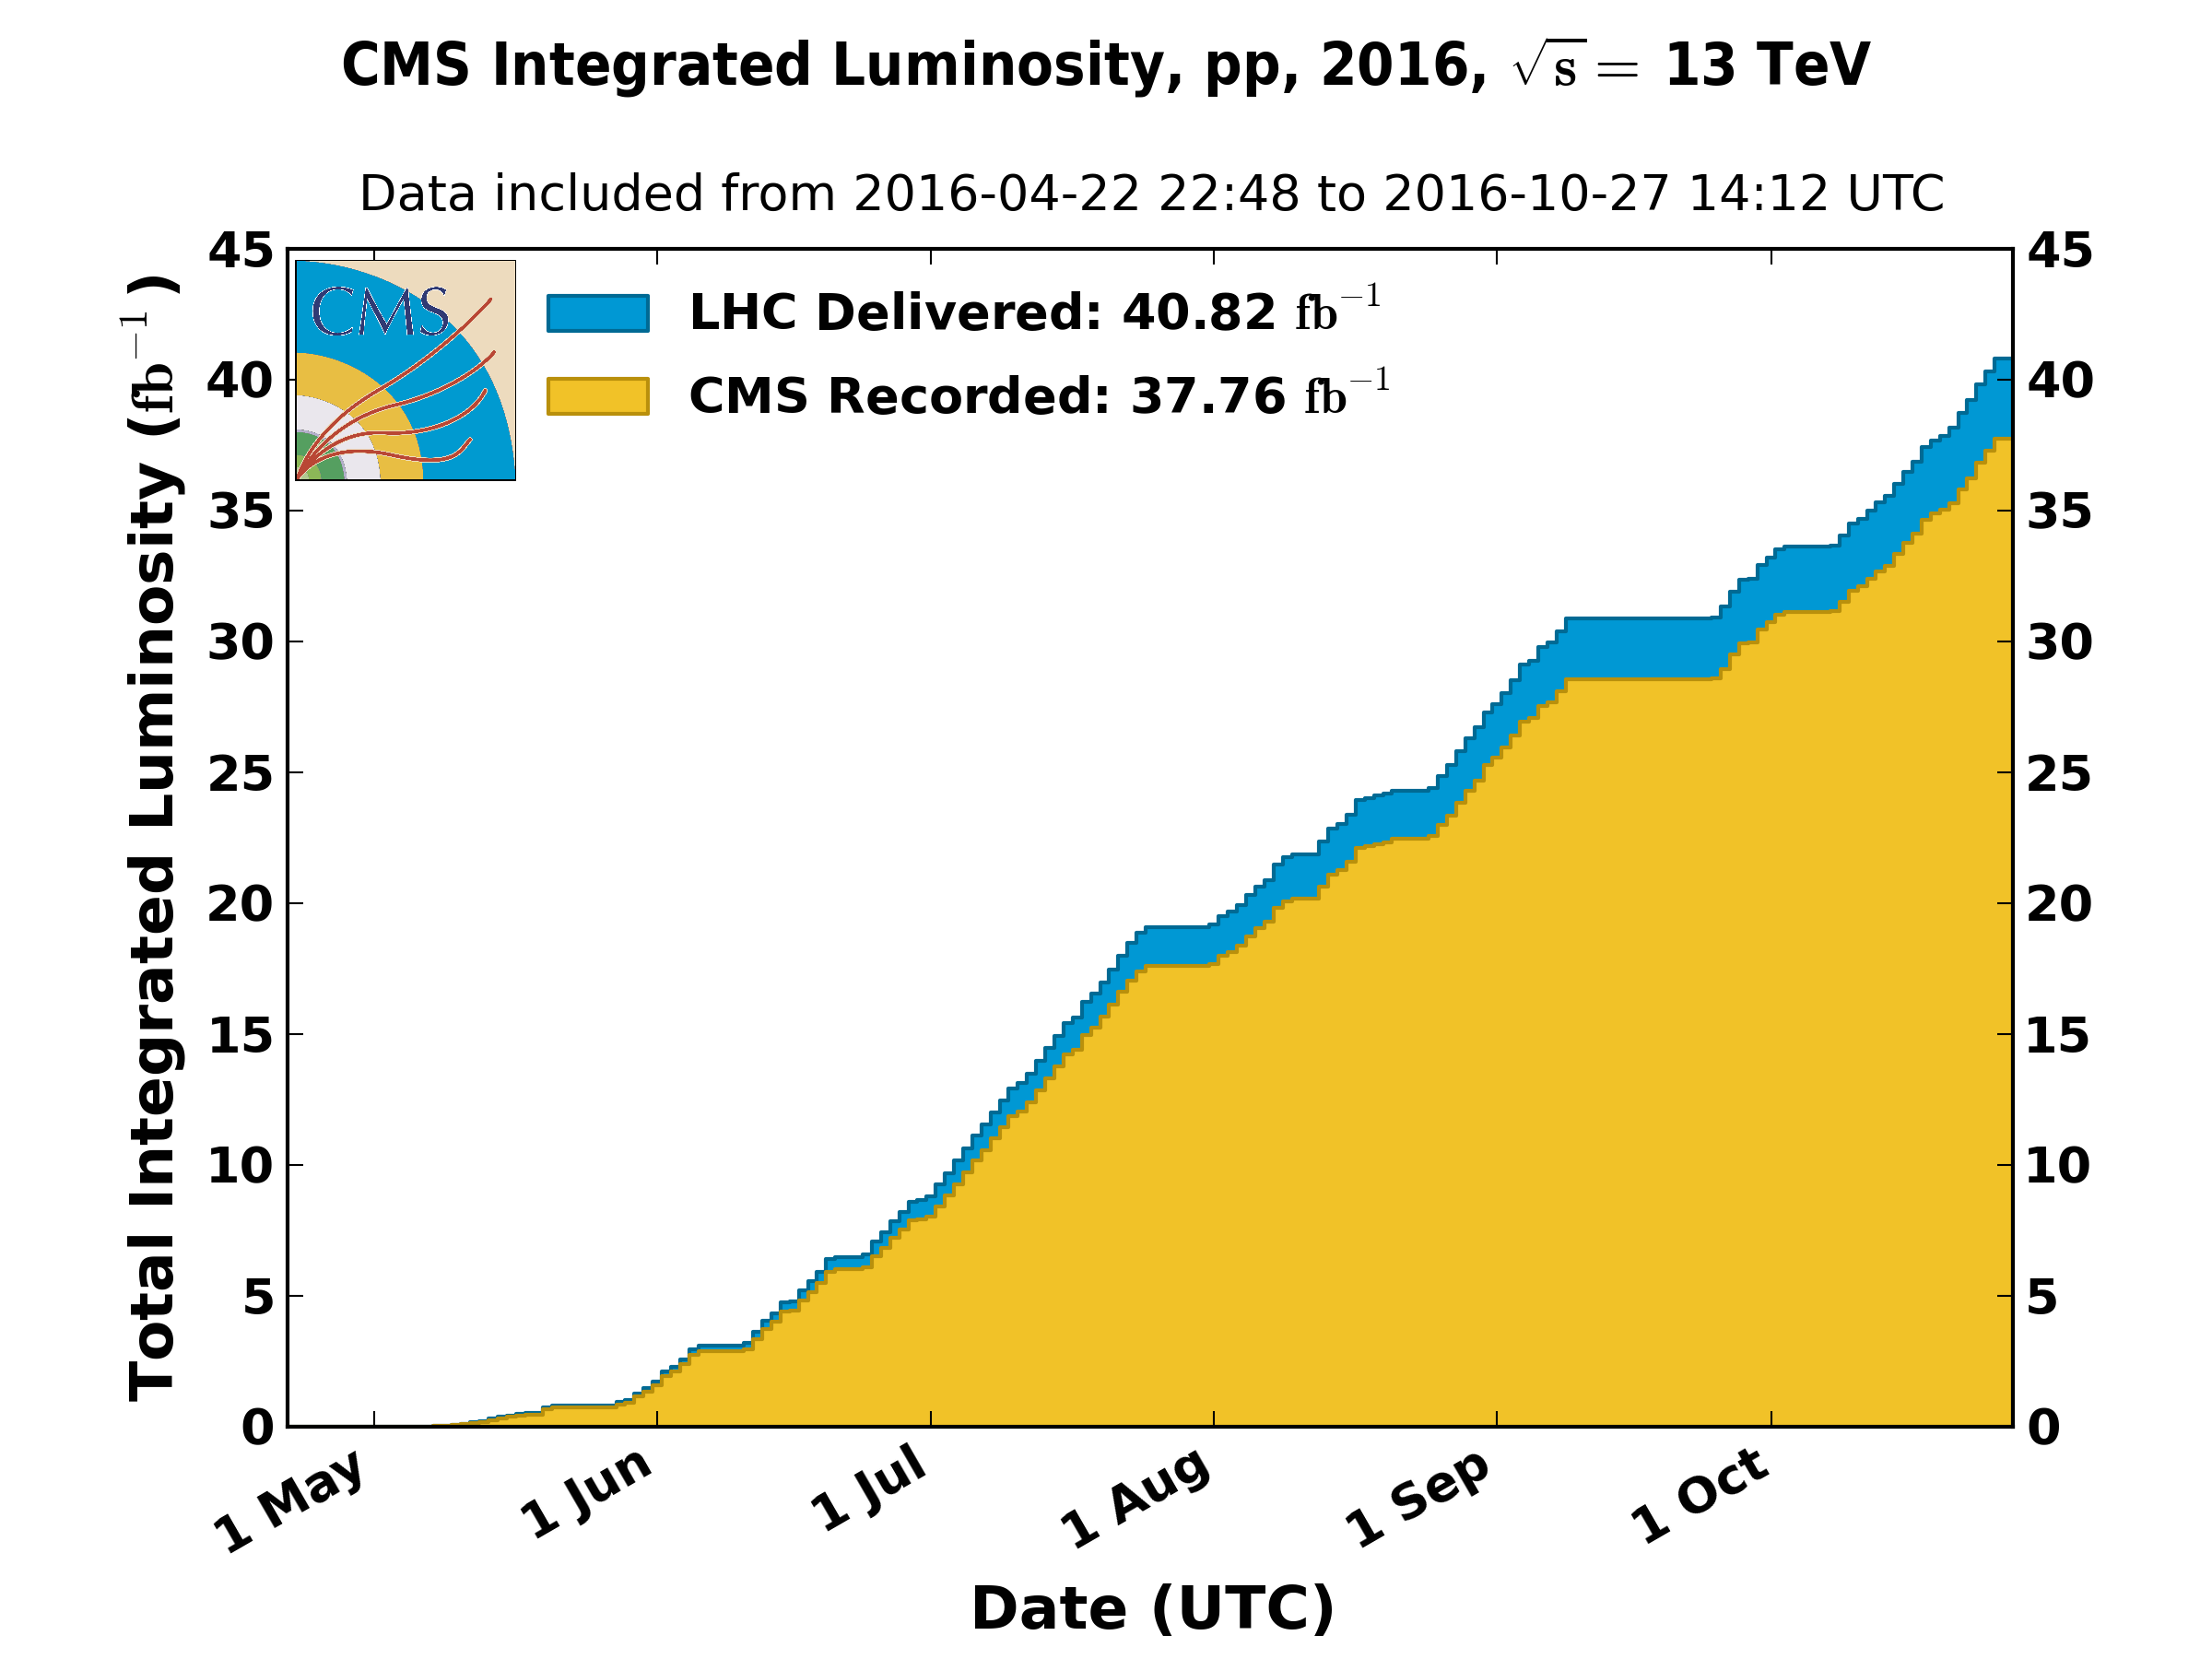
\includegraphics[width=0.4\textwidth,keepaspectratio]{plots_and_figures/chapter3/int_lumi_per_day_cumulative_pp_2016.png}
\caption{Evolution of integrated luminosity in 2015 and 2016 delivered by LHC (blue), and collected by CMS detector (orange)~\cite{cms_int_lumi_ref}.}
\label{fig:cms_int_lumi}
\end{center}
\end{figure*}

In the longer term, it is planned to keep the LHC running, punctuated with several scheduled stops for upgrades and maintenance, at least until late 2030s. During this period it is anticipated to operate at increasingly higher luminosities helping collect unprecedented amounts of data. Figure~\ref{fig:lhc_schedule} shows an overview of the long term LHC schedule. 
\begin{figure*}
\begin{center}
  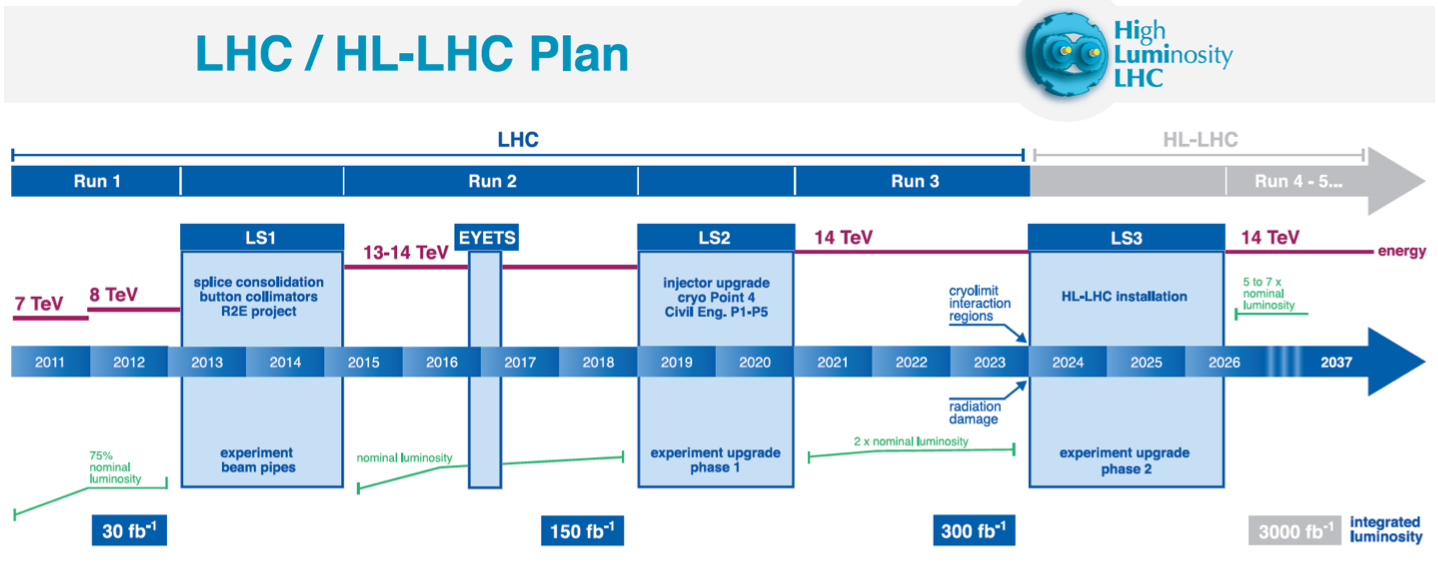
\includegraphics[width=0.95\textwidth,keepaspectratio]{plots_and_figures/chapter3/lhc_schedule.png}
\caption{Overview of the long term LHC schecdule~\cite{LHC_plan_ref}.}
\label{fig:lhc_schedule}
\end{center}
\end{figure*}



\section{The CMS Detector}
\label{sec:CMS}
The Compact Muon Solenoid~\cite{cms_exp_ref} is a general multipurpose particle physics detector that is placed in one of the four collision points of the LHC. It is 28.7\,m long with a diameter of 15.0\,m, weighs 14000 tonnes, and is composed of several subdetectors. Its aim is to study a broad array of physics, from making precise measurements of known processess to searches for exotic processes predicted by a multitude of BSM theories. In order to be able to pursue its physics aims at the challenging LHC conditions, the CMS experiment needs to meet several requirements which primarily include good muon identification and momentum resolution over a wide range of momenta and angles, good dimuon mass resolution, good charged-particle momentum resolution and reconstruction efficiency, good electromagnetic energy resolution, good diphoton and dielectron mass resolution, good missing-transverse-energy and dijet-mass resolution.
The backbone of the CMS is a superconducting solenoid that houses its tracking and calorimetry systems and provides an axial magnetic field of 3.8\,T. The inner-most layer is the silicon pixel and strip tracker that measures the trajectories of charged particles. Surrounding the tracker are the lead tungstate crystal electromagnetic calorimeter (ECAL) which measures the energy of electrons and photons, and the hadronic calorimeter (HCAL) which measures the energy of heavier particles that pass through the ECAL. The ECAL also contains a preshower detector for extra spatial precision. Outside the solenoid is the muon system which has gas-ionization detectors placed in the steel yoke of the magnet. This is the outermost component of CMS and measures the momenta of muons that traverse through it. A sophisticated two-level trigger system that helps filter out a small fraction of most interesting events among millions produced at the LHC also forms a vital part of the CMS. The powerful solenoid, sophisticated muon system and its compact design (given its complexity) give CMS its name. Figure~\ref{fig:cms_layered} shows a layered view of the detector. Figure~\ref{fig:cms_cross_sec} shows a transverse cross-sectional view along with specific paticle interactions. The following sections describe the detector in further detail.   

\begin{figure*}
\begin{center}
  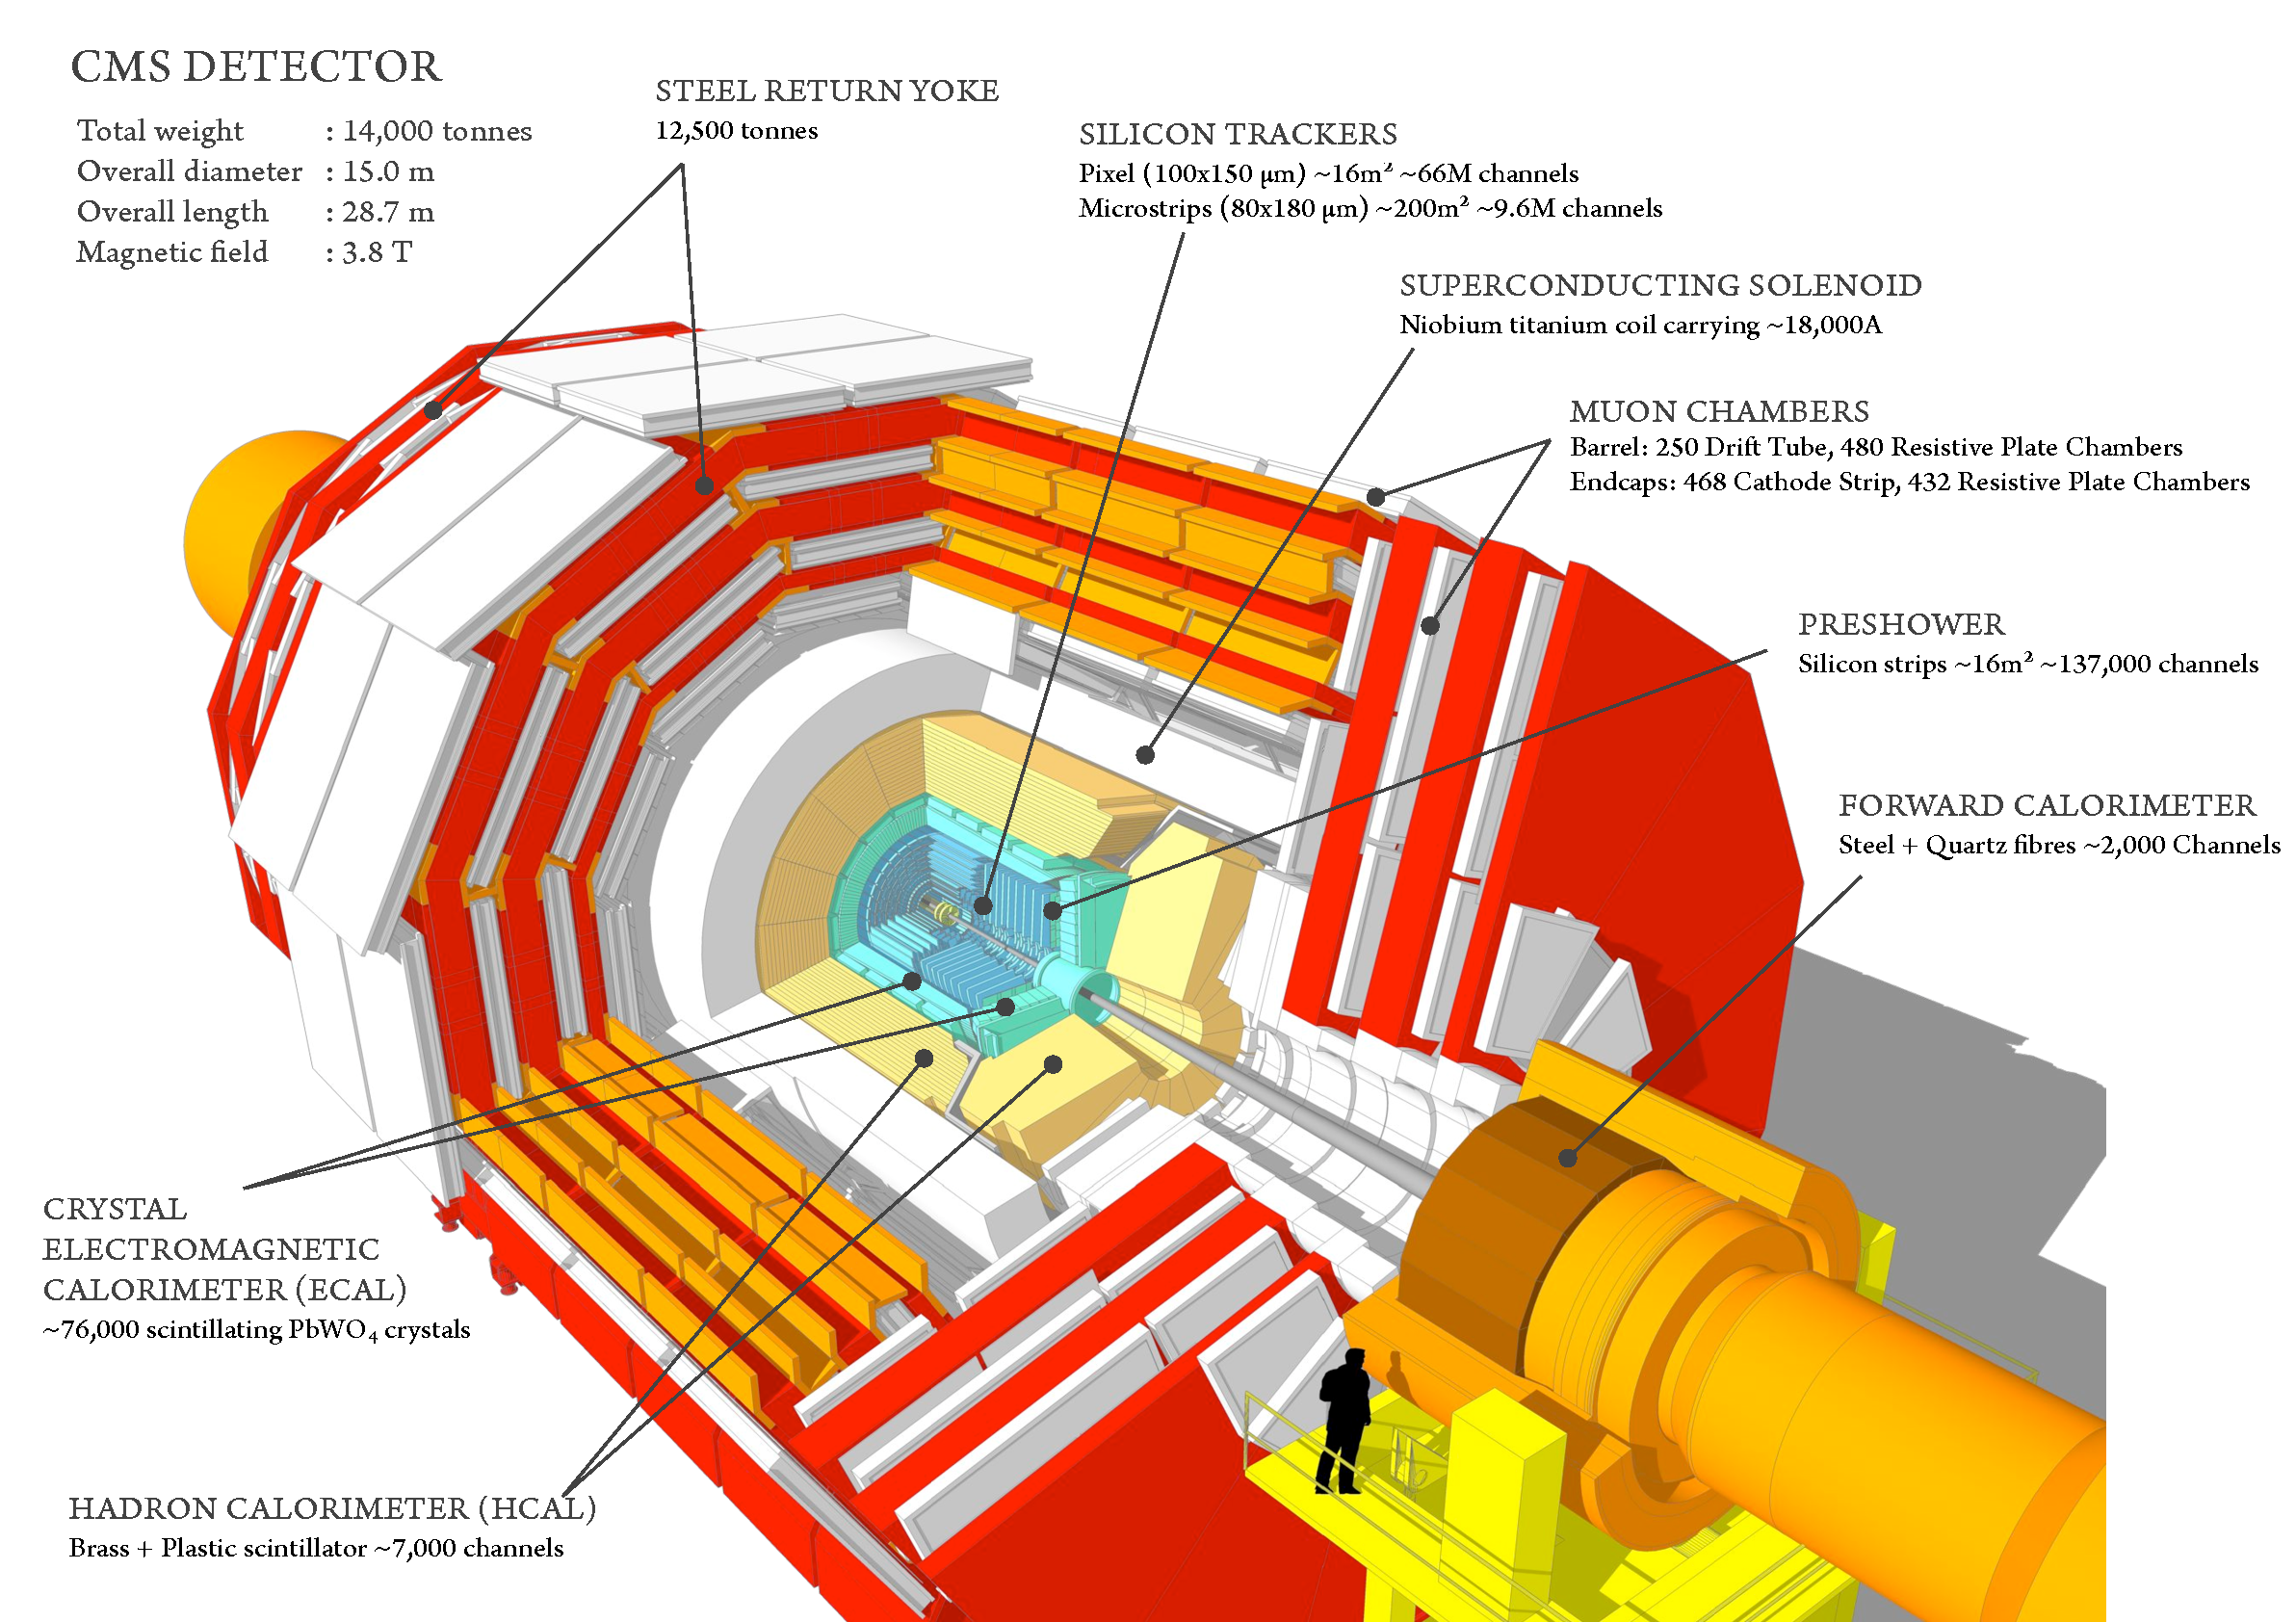
\includegraphics[width=0.95\textwidth,keepaspectratio]{plots_and_figures/chapter3/cms_layered.png}
\caption{Layered View of the CMS detector}
\label{fig:cms_layered}
\end{center}
\end{figure*}



\begin{figure*}
\begin{center}
  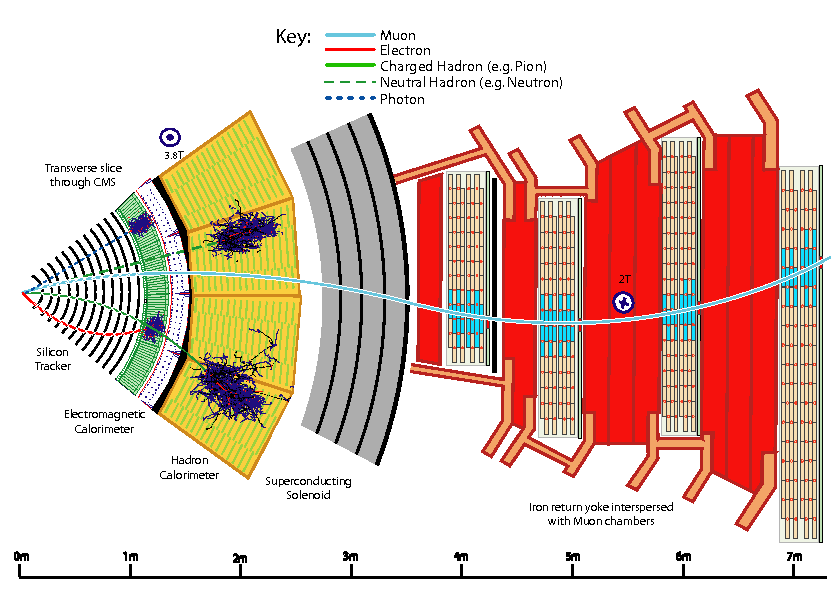
\includegraphics[width=0.95\textwidth,keepaspectratio]{plots_and_figures/chapter3/cms_cross_sec.png}
\caption{Transverse cross-sectional view of the CMS along with specific particle interactions~\cite{Sirunyan:2017ulk}.}
\label{fig:cms_cross_sec}
\end{center}
\end{figure*}




\subsection{Coordinate Conventions}
\label{cor_conv}
The CMS detector has adopted a right-handed coordinate system, the origin of which lies at the nominal collision point inside the experiment. The x-axis points radially inward towards the center of the LHC while the y-axis points vertically upwards. This makes the z-axis point along the beam direction. At point 5 of LHC (a village named Cessy in France) where the CMS is, the z axis points toward the Jura Mountains. In cylindrical co-ordinates, the polar angle $\theta$ is measured from the z-axis while the azimuthal angle $\phi$ is measured from the x-axis in the x-y plane. The polar angle is used to define the pseudo-rapidity $\eta =-ln(tan(\frac{\theta}{2}))$, which is a close approximation for rapidity if $E\gg m$. The rapidity is a Lorentz invariant quantity under boosts in the z-direction. Since it is typical of particles that CMS sees to have $E\gg m$, the Lorentz invariance approximately holds for pseudo-rapidity as well. 


\subsection{Charged Particle Tracking System}
\label{tracker}
The Charged Particle Tracking system or the tracker measures, efficiently and precisely, the trajectories of charged particles passing through it~\cite{cms_exp_ref, pix_det, pix_det2}. It is cylindrical in shape with a length of 5.8\,m and diameter of 2.5\,m. The momentum of charged particles can be measured using these tracks with high precision. The tracker also helps in reconstruction of secondary vertices of lon-lived particles. Given the tracker is innermost layer of the CMS and the challenging LHC conditions, the tracker experiences high particle flux. Therefor, the material it is built of needs to be radiation hard. This makes silicon a good choice for detector material. The tracker also needs to be highly granular and have fast response in order to be able to efficiently and precisely measure the trajectories. However, it is also necessary to keep the amount of material of the tracker low to limit photon conversion, multiple scattering, bremsstrahlung and nuclear interactions. A compromise between these two aspects led to the current design of the tracker whcih consists of two subsystems. The inner layer consists of a detector made of 66 million silicon pixels. They pixels are 100\,$\mu$m$\times$150\,$\mu$m and arranged in the form of three barrel layers with radii of 4.3\,cm, 7.2\,cm and 11 cm respectively, and two endcap disks on each side of the barrel at 34.5\,cm and 46.5\,cm from the interaction point. Figure~\ref{fig:pix_det} shows illustrations of the CMS pixel system and that of a section showing a pixel element. Outside the region of the pixel detector, the density of tracks is low and the high granularity requirment can be somewhat relaxed. The outer subsystem of the tracker is thus made of strips of silicon. The strip detector consists of 10 barrel layers which are organized into 4 inner layers, called Tracker Inner Barrel (TIB) and 6 outer layers, called Tracker Outer Barrel (TOB). They range in radii from 25\,cm to 110\,cm. It also consists of 12 endcap disks on each side of the barrel which have radii upto 110\,cm, and are up to 280\,cm from the interaction point. They are organized on each side into 3 inner endcap disks, called Tracker Inner Disks (TID) and 9 outer disks, called Tracker End Cap (TEC). Figure~\ref{fig:tracker_layout} shows the layout of the tracker subsystems.    

\begin{figure*}
\begin{center}
  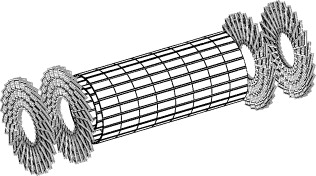
\includegraphics[width=0.85\textwidth,keepaspectratio]{plots_and_figures/chapter3/pixeldet.jpg}
  \\
  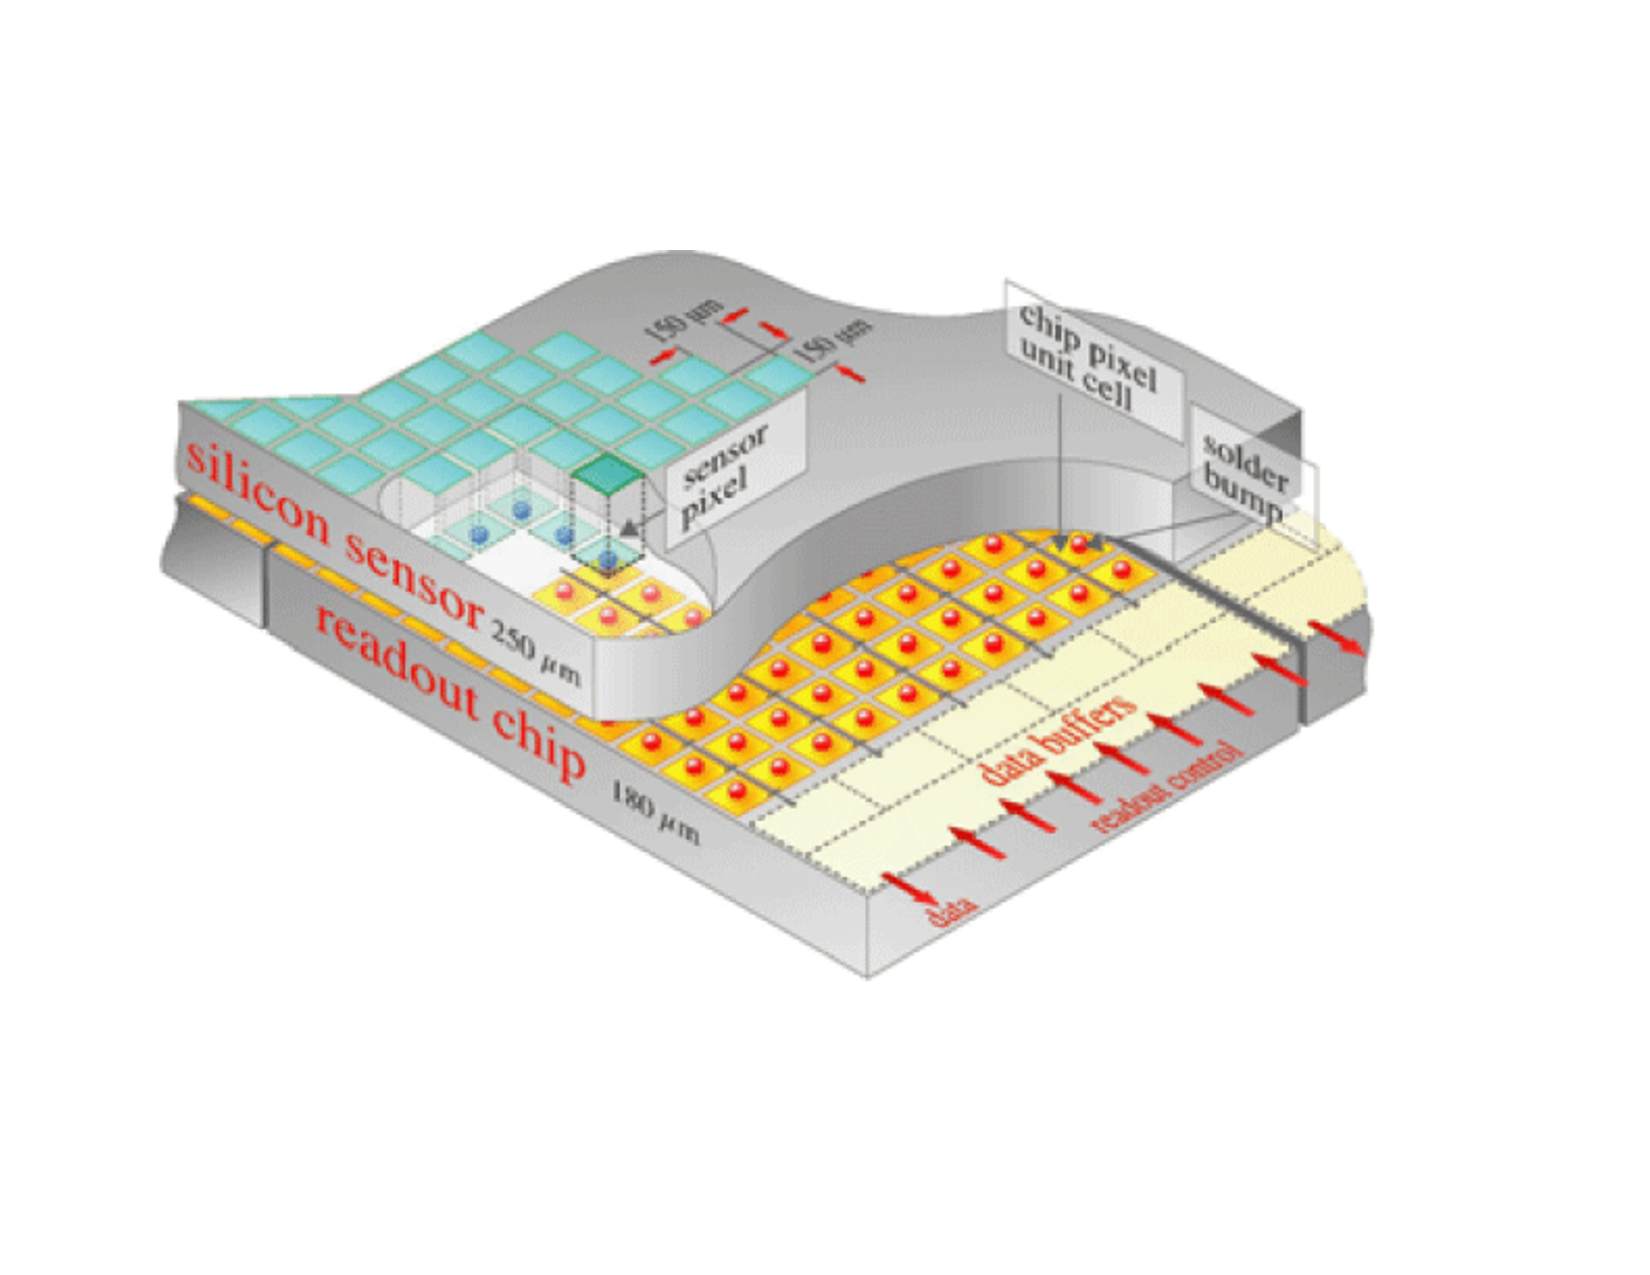
\includegraphics[width=0.7\textwidth,keepaspectratio]{plots_and_figures/chapter3/pixelelem.pdf}
\caption{Perspective view of the CMS pixel detector (top)~\cite{pix_det}, and illustration of a section showing individual pixel elements (bottom)~\cite{pix_elem}.}
\label{fig:pix_det}
\end{center}
\end{figure*}


\begin{figure*}
\begin{center}
  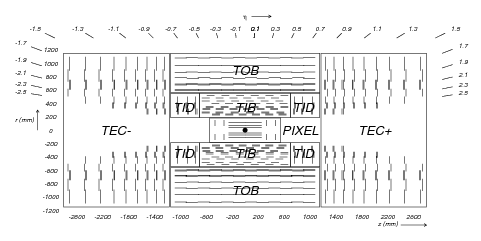
\includegraphics[width=0.98\textwidth,keepaspectratio]{plots_and_figures/chapter3/trackerlayout.png}
\caption{The CMS tracker layout~\cite{cms_exp_ref}.}
\label{fig:tracker_layout}
\end{center}
\end{figure*}

The combination of the pixel and strip trackers give the CMS excellent track resolution and efficieny. The algorithm used to reconstruct these tracks from hits in the pixels and strip detectors is described in detail in Section~\ref{track_recon}.  Promptly  produced,  isolated  muons  of $pT>0.9$\,GeV are reconstructed with close to 100\% efficiency for $|\eta|<2.4$~\cite{track_reconstruction}. The transverse momentum resolution for 100\,GeV muons in the central region of $|\eta|<1.4$ is about 2.8\%, while the impact parameter resolution is about 10$\mu$m and 30$\mu$m in the transverse and longitudinal directions.


\subsection{Electromagnetic Calorimeter}
\label{Ecal}
The Electromagnetic Calorimeter or ECAL is the next layer of the CMS detector. It fits snugly in between the tracker and the HCAL (next section) and measures the energy of electrons and photons. Besides being a important for many other interesting analysis, one of the two final state particle in the searches described here is an electron. The ECAL is a homogenous calorimeter; the absorber and scintillator materials are one and the same. In other words, the entire volume of the calorimeter can potentially contribute towards a signal. This does away with the error introduced by sampling (which is needed in case of calorimeters which are not homogenous). The material chosen for the ECAL is Lead Tungstate ($\mathrm{PbWO}_4$), which despite being heavier (density=$8.3\,\mathrm{g/cm}^3$) than stainless steel (density$<8\,\mathrm{g/cm}^3$) is highly tranparent in its crystalline form. The $\mathrm{PbWO}_4$ crystals (Figure~\ref{fig:ecal_crystal}) used in the ECAL are 23 (22)\,cm in length and $2.2\times2.2\,(2.86\times2.86)$\,cm in tranverse size for the barrel (endcap)~\cite{ecal2}. These high density crystals have a short radiation length ($\mathrm{X}_{\circ}=0.85$\,cm) and a small Moli\'ere radius ($\mathrm{R}_{M}=2.19$\,cm). The radiation length of a material is the mean distance over which an incident electron loses all but 1/e of its energy, or 7/9 of the mean free path for pair production by a high energy photon. Electromagnetic showers are intiated in the ECAL when a high energy electron or photon enters its volume. An electron emits photons via bremsstrahlung radiation. These photons in turn pair produce electron-poistron pairs which can in turn release more photons. This stops when the photon energy becomes lower than what is required for pair production (usually a few MeV). The ``depth'' of an electromagnetic shower scales logarithmically with energy and linearly with radiation length. Therefore, having a short radiation length is important. Since, the length of $\mathrm{PbWO}_4$ crystals (23\,cm) used in the ECAL is about 27 times the radiation length (0.85\,cm), they are able to contain full showers. Another important quantity, the Moli\'ere radius is the radius of the cylinder that contains 90\% of shower in the lateral direction. The small Moli\'ere radius ($2.19\,cm$) of $\mathrm{PbWO}_4$ thus helps the ECAL in delivering a high position resolution. Further, these crystals also produce light fast with 80\% of light being emitted in 25\,ns (LHC bunch crossing time). Because this light yield depends strongly on temperature ($-2\%/^{\circ}C\,\mathrm{at}\,18^{\circ}C$), it is necessary to maintain the ECAL at a constant temperature ($18\pm0.05^{\circ}C$). Also, despite being radiation hard, the crystals still suffer from reduction of transparency due to irradiation. Damage and recovery of the crystals is measured using laser light (Figure~\ref{fig:ecal_las_corr}), and this is corrected for periodically in measurements made by the ECAL.     
\begin{figure*}
\begin{center}
  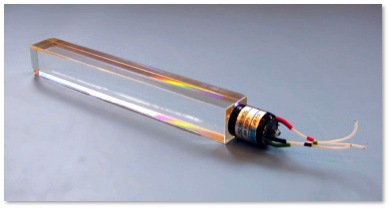
\includegraphics[width=0.7\textwidth,keepaspectratio]{plots_and_figures/chapter3/crystal.jpg}
\caption{A $\mathrm{PbWO}_4$ ECAL crystal~\cite{ecal1}.}
\label{fig:ecal_crystal}
\end{center}
\end{figure*}

\begin{figure*}
\begin{center}
  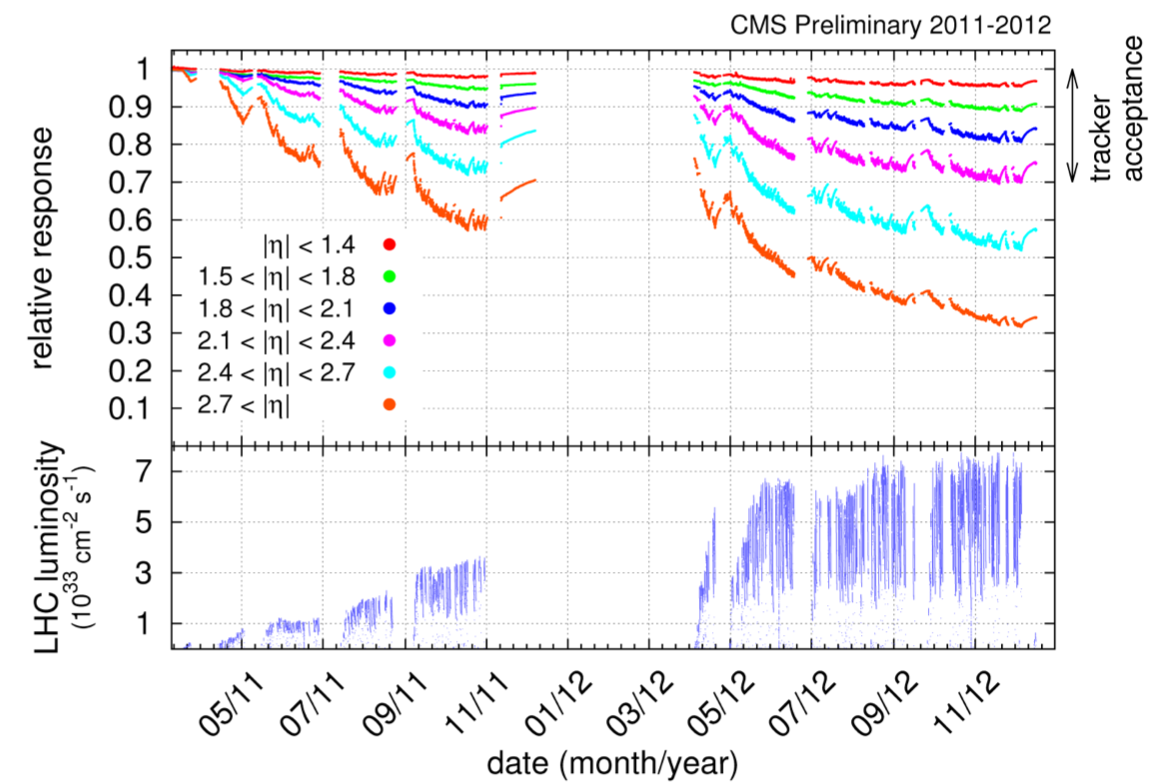
\includegraphics[width=0.8\textwidth,keepaspectratio]{plots_and_figures/chapter3/ecal_laser_corr.png}
\caption{Relative response loss of ECAL due to radiation effects, as function of time in different $\eta$ regions as measured by the laser monitoring system~\cite{ecal2}.}
\label{fig:ecal_las_corr}
\end{center}
\end{figure*}

The crystals of the ECAL are organized into a barrel and two endcaps, one on each side. The layout is illustrated in Figure~\ref{fig:ecal_layout}. The barrel extends up to $|\eta|<1.479$ and is made of 61200 crystals, which are further organized into 36 supermodues of 1700 crystals each. The endcaps cover the region between  $1.65<|\eta|<3.0$, and are each made of two Dees with 3,662 crystals in each Dee. The 75,848 crystals together weigh 92 tonnes. The crystals are equipped with photodetectors which convert the light output to amplified electrical signals. In the barrel each crystal is equipped with two $5\times5\,\mathrm{mm}^2$ APDs (Avalanche Photo Diodes) which have a gain of 50. In the endcaps, the radiation is too high to use silicon photodiodes. Here, VPTs (Vacuum Phototriodes), with a gain of $\sim$10, are used instead. Each endcap crystal has a VPT glued to the end of it (as seen in Figure~\ref{fig:ecal_crystal}). The energy resolution of the ECAL can be parametrized as the sum of a stochastic term, a noise term and a constant term. The resolution depends on energy, and for the ECAL barrel this is can be approximated by: $(\frac{\sigma}{E})^2=(\frac{0.028}{\sqrt{E}})^2+(\frac{0.12}{E})+0.003^2$~\cite{ecal3}.

\begin{figure*}
\begin{center}
  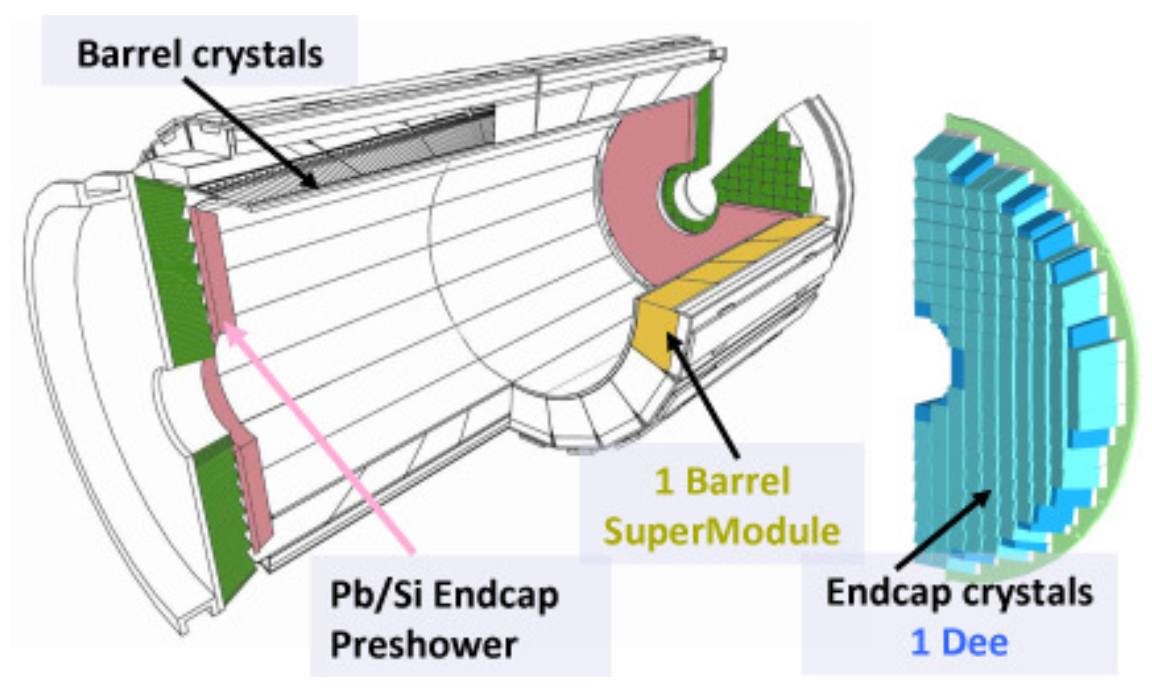
\includegraphics[width=0.9\textwidth,keepaspectratio]{plots_and_figures/chapter3/ecal_layout.png}
\caption{CMS ECAL layout~\cite{ecal2}.}
\label{fig:ecal_layout}
\end{center}
\end{figure*}

I worked closely with the ECAL during the time spent at CERN. The next subsection briefly describes a project related to the ECAL that I worked on.

\subsubsection{Mitigation of anomalous APD signals in the ECAL barrel}
As mentioned in the last section, APDs are used as photodetectors to collect, amplify and convert light to electronic signals in the barrel section of the ECAL. The APDs use silicon as active element and have an active area of $5\times5\mathrm{mm}^2$. Each ECAL crystal has a pair of APDs. Figure~\ref{fig:apd} shows an ECAL APD mounted in a module. The APDs suffer from a problem which can be considered both strange and interesting in nature. Particles produced in the collisions (usually neutrons) can ocassionally strike the APDs directly and interact with the material, that cause large depsits through direct ionization of the silicon~\cite{petyt}. These deposits cause anomalous signals to be registered as coming from a real electron or photon that has scintillated the ECAL. These anomlaous signals are usually called 'spikes', and they can range from a few GeV to to a few hundred GeV in energy. When the collected data is being processed, these  depsoits must be eliminated with high accuracy and efficiency for subsequent analysis. This is called offline rejection, an algorithm called the swiss-cross algorithm along with timing information is used to get rid of these deposits with almost cent percent eficiency. However, offline rejection of spikes is not enough. Because spikes are produced at a rate proportional to number of collisions, at a high luminosity output collider like the LHC, spikes cause problems with triggering, as they 'eat up' the $\sim100\,$kHz bandwidth available at the first level of triggering (see section~\ref{trigger} for a description of the two-level CMS trigger system). Thus a majority of spikes need to be eliminated 'online', that is when the data is being collected live. Given that the hardware based first level of the CMS trigger (L1) has only 3.2\,$\mu$s to make a decision, spikes need to be identified and rejected fast in the firmware.     

\begin{figure*}
\begin{center}
  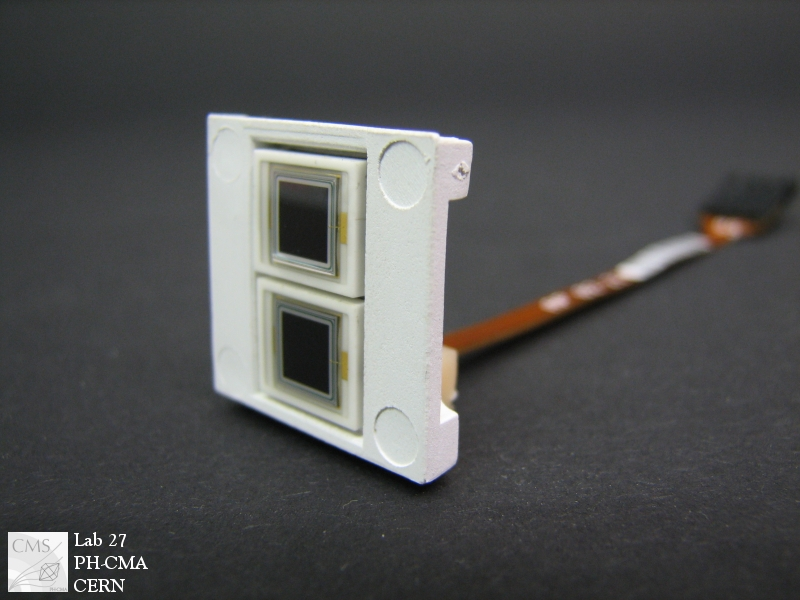
\includegraphics[width=0.6\textwidth,keepaspectratio]{plots_and_figures/chapter3/apd.jpg}
\caption{Two CMS ECAL Avalanche Photodiodes~\cite{apd}.}
\label{fig:apd}
\end{center}
\end{figure*}

Spikes masquerade well as true electromagnetic (EM) energy deposits. However, the defining charecteristic of spikes is that they deposit all their energy in a single ECAL crystal. In contrast, as mentioned in the last section, EM showers spread. The spread is even larger in the direction perpendicular to the magnetic field ($\phi$-direction). A well-centered EM shower deposits about $\sim80\%$ of its energy (E1) in the central crystal. However, the remaining $\sim20\%$ of its energy is spread in a neighboring crystal. Based on the above ideas, a discriminating variable is defined as $1-\frac{E4}{E1}$, where E4 is the energy deposited in the 4 nearest neighbors of the central crystal. This variable is named the 'Swiss-cross' variable. Figure~\ref{fig:swisscross} (left) shows how the Swiss-cross variable is defined. The distribution of this variable is shown Figure~\ref{fig:swisscross} (right), for data collected from pp collisions and Monte-Carlo simulated data contaning only EM energy deposits. A secondary peak at high Swiss-cross values can be clearly seen in only the pp collision data, and corresponds to spikes. Thus, this variable can be used to discriminate very well against spikes. In fact $99\%$ spikes can be rejected using this variable alone. This can be further improved by using other characteristics such as pulse shape and timing that separate spikes from EM deposits.


\begin{figure*}
\begin{center}
  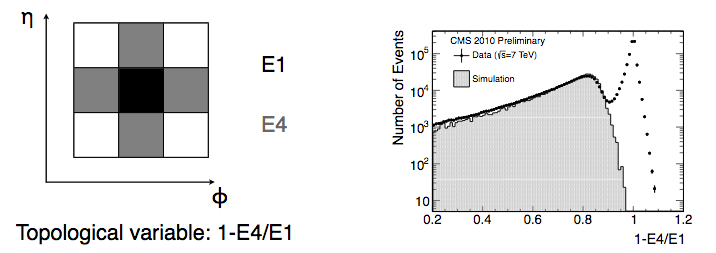
\includegraphics[width=0.9\textwidth,keepaspectratio]{plots_and_figures/chapter3/swisscross.png}
\caption{Definiton of the Swiss-cross variable (left) and its distribution in pp collision data and simulated EM events~\cite{petyt}.}
\label{fig:swisscross}
\end{center}
\end{figure*}

Although the Swiss-cross algorithm described above is relatively simple, it still isn't possible to implement in online and run it on firmware under the 3.2\,$\mu$s od time that the L1 trigger has to make a decision. Therefore, a much simpler adaptation of the Swiss-cross algorithm was implemented. This algorithm exploits the fact that the EM showers spread in the $\phi$ direction due to the magnetic field. The smallest building block of an EM candidate, i.e. an electron or a photon, is a trigger tower (TT). A TT is a block of $5\times5$ crystals in the $\eta\times\phi$ direction. These TTs are send downstream by L1 trigger to the next triggering level (HLT, see section~\ref{trigger}). A base block associated with a TT is called a trigger primitive (TP). The aim of this algorithm is to thus reduce the proportion of TPs induced by spikes within a short amount of time available. For each of the 5 $1\times5$ strips lengthwise across the $phi$ direction in a TT, the number of crystals  having energy above a certain threshold is counted. If in any of this strips more than 1 channel is above the threshold (hopefully owing to EM shower spread), a logic flag called the sFGVB (strip Fine Grain Veto Bit) is set to 1. Otherwise, it is set to 0. A TP with sFGVB 0 is considered to have been induced by a spike and is discarded. Not all TPs are subject to the above rule. Only TP with total energy above a certain threshold are eliminated. Otherwise, we would end up discarded many real low energy EM candidates thereby reducing the overall efficiency of detecting such candidates. The sFGVB threshold mentioned earlier is $\eta$ dependent, and its average value corresponded to 350\,MeV in run I while TP-killing threshold was set at 12\,GeV. Using this algorithm, the proportion of spike-induced TPs were kept low in run I ($\sim15\%$).      


\begin{figure*}
\begin{center}
  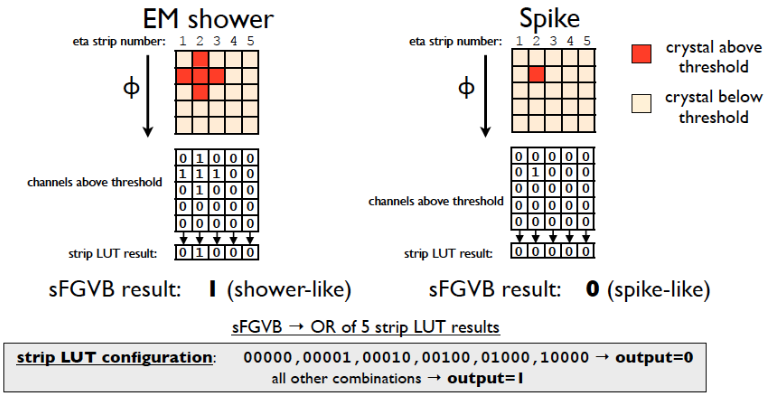
\includegraphics[width=0.95\textwidth,keepaspectratio]{plots_and_figures/chapter3/sfgvb.png}
\caption{Illustration of the Strip Fine Grain Veto Bit~\cite{sfgvb}.}
\label{fig:swisscross}
\end{center}
\end{figure*}

LHC conditions have become more an more challenging since the start of Run II in 2015. The instantaneous luminosity has risen continuously, and the bunch crossing has been reduced to 25\,ns. This means CMS can now collect a lot more data at a faster rate which is great. However, this also means the ECAL APDs get hit with much more spikes compared to RUN I. In data collected in 2015 and early 2016, this effect was observed as expected. This is shown in Figure~\ref{fig:spike_fraction}. The proportion of spike induced TPs had increased progressively, and the online spike rejection algorithm needed to be tuned to the newer LHC conditions.    


\begin{figure*}
\begin{center}
  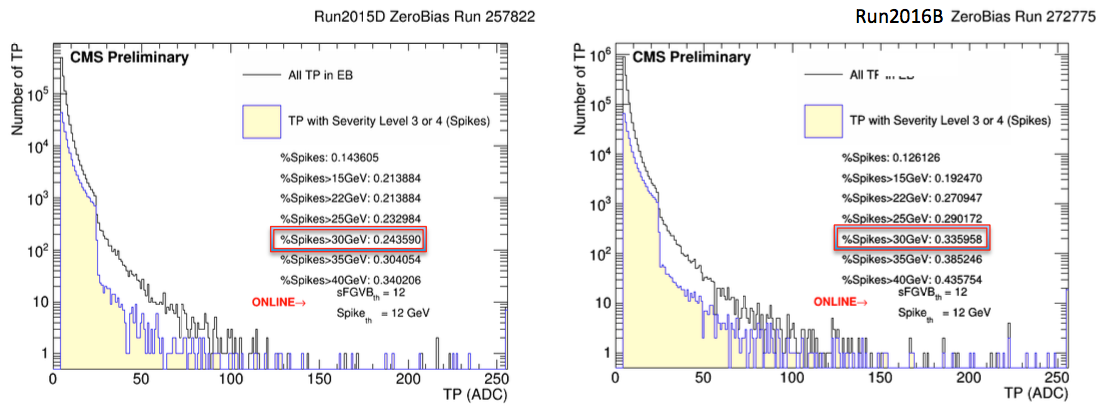
\includegraphics[width=0.95\textwidth,keepaspectratio]{plots_and_figures/chapter3/spike_fraction.png}
\caption{Spectrum of energy for all TPs (black line) and TPs induced by spikes (blue line with yellow fill) for pp collison runs from 2015 (left) and 2016 (right). Percentage of spike induced contamination above different energy thresholds are also noted.}
\label{fig:spike_fraction}
\end{center}
\end{figure*}

There are several things that need to be considered when tuning the above algorithm. The spike contamination should go down, however this should not come at the cost of reduction in efficiency of detection real EM candidates. Further, the overarching L1 triggering rate should not increase, and if possible decrease. Therefore, in order to tune the algorithm one needs to adjust both thresholds: sFGVB threshold and the TP-killing threshold. Simply increasing the sFGVB threshold would eliminate more spikes, but it would also end of rejecting some real EM candidates. Thus, in order to keep the efficiency of EM candidate detection good, we need to increase the TP-killing threshold as well. An array of working points (possible values for the thresholds) were studied. They ranged from 14 to 22\,GeV for the TP-killing threshold, and $\sim400$to$\sim900\,$MeV for the sFGVB threshold. For each of these working points, the residual contamination from spikes was calculated. The efficiency for detection of EM candidates was also calculated. Figure~\ref{fig:spikeroc} shows the purity (1-proportion of spike contaminated TPS), i.e. proportion of real EM candidates  plotted v/s EM candidate efficiency, for various working points. The ideal working point would corresponding to the point closest to the top right corner of the plot. However, we would also need to consider the third factor mentioned above, i.e. the triggering rate. Increasing the TP-killing threshold increases the rate at which all triggers below that threshold fire (slect events). However, each increasing TP-killing threshold is accompanied by a higher sFGVB threshold which brings the rate of firing of all triggers above the TP-killing threshold down. The L1 rate for each of the working points being studied were also calculated. The optimal working point would thus have a higher rate decrease and a lower rate increase thus bringing the overall L1 triggering rate down, and keeping spike contamination low and EM candidae selction efficiency high.

\begin{figure*}
\begin{center}
  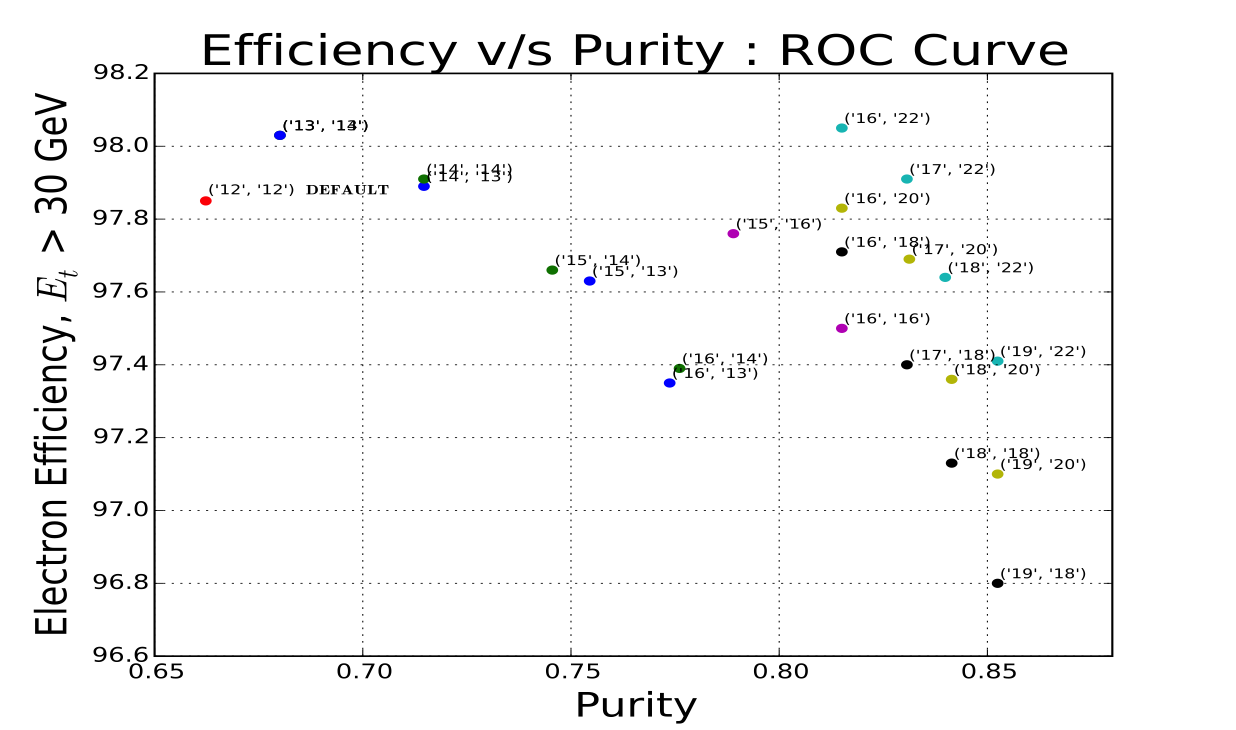
\includegraphics[width=0.95\textwidth,keepaspectratio]{plots_and_figures/chapter3/spikeroc.png}
\caption{Purity (proportion of TPs which are not spike induced) v/s efficiency of selection of EM candidates. }
\label{fig:spikeroc}
\end{center}
\end{figure*}

Based on all the aforementioned factors, the new thresholds chosen were $~500\,$MeV for sFGVB and 16\,GeV for TP-killing. The tuned spike rejection algorithm was able to reduce the contamination rate down to acceptable levels, and reduce the overall L1 trigger rate from EM candidates.  

%\subsubsection{ML-driven anomaly detection for the ECAL DQM}


\subsection{Hadronic Calorimeter}
\label{Hcal}
The Hadronic Calorimeter (HCAL) is designed to detect and measure the energy of particles that interact via the strong force~\cite{cms_exp_ref}. In CMS, this typically means hadrons. In addition, it is also indirectly responsible for measurement of missing transverse energy, $\ptvecmiss$ (see~\ref{mt_met_recon}). The $\ptvecmiss$ is calculated from imbalance in momentum in the transverse direction, and helps measure the energy of neutrinos, or other such particles, which do not interact with the CMS. In order to help measure $\ptvecmiss$ accurately, the HCAL needs to be hermetic, i.e. it should effectively capture each and every particle produced in the collision irrespective of the region in which it is produced. Unlike the ECAL which is homogeneous, the HCAL belongs to a different class of calorimeters called sampling calorimeters~\cite{hcal1}. In such calorimeters, the  material that produces light and measures energy (scintillator) is different from the material that produces the particle shower (absorber). It is chosen to be made of repeating layers of dense absorber and tiles of plastic scintillator. The dense absorber tiles are made of brass and steel. Hadrons interact with absorber plates to produce numerous secondary particles. These secondary particles interact with successive layers of absorber to give rise to a hadron shower. When the shower passes through the plastic scintillator layers alternating with absorber, it causes the scintillating material to emit light. This light is collected by optical fibers that are embedded within each scintillator tile, and then sent to photosensors. The photosensors used in the HCAL are fast and radiation resistant, and convert the light to electronic signals. The energy deposited can then be measured using these signals. Obviously, because of the absorber layers, the entire energy deposited is not converted into electronic signals. However, we can estimate the total energy deposited in the calorimeter from the energy collected by sampling (and hence the name sampling calorimeter) the shower (using  energy deposited) in several layers of scintillator.

%If the HCAL were a homogeneous calorimeter we would need a very large material budget, because hadrons would pass through much larger amounts of scintillating material compared to what electrons and photons pass through in the ECAL. Besides the fact that a large amount of scintillating material is very expensive, there is not enough room between the ECAL and the magnet for the HCAL to be made homogeneous. Thus, the HCAL


\begin{figure*}
\begin{center}
  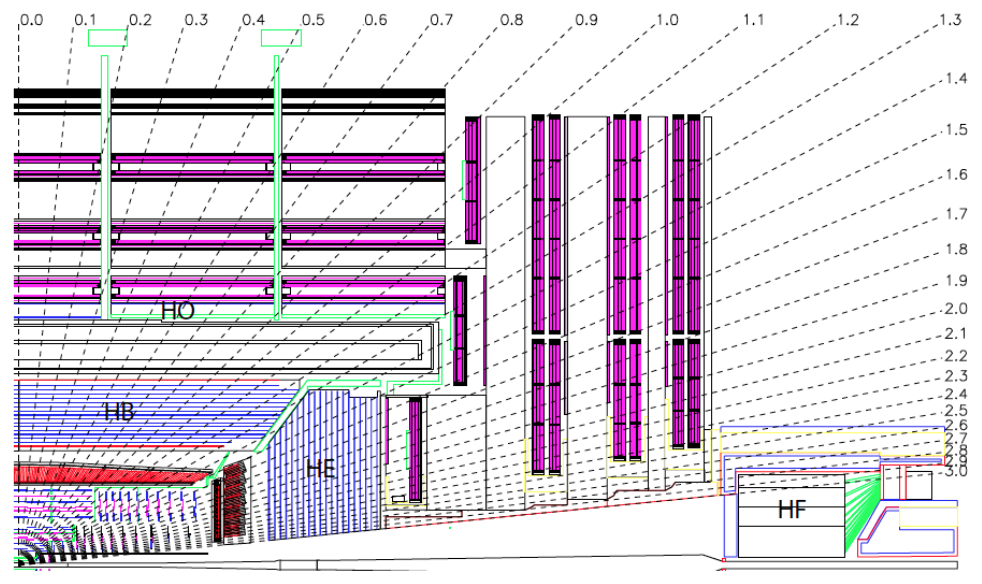
\includegraphics[width=0.98\textwidth,keepaspectratio]{plots_and_figures/chapter3/hcal_layout.png}
\caption{The CMS HCAL layout~\cite{cms_exp_ref}.}
\label{fig:hcal_layout}
\end{center}
\end{figure*}

Like all other CMS subdetectors, the layout of the HCAL is also very modular and divided into four distinct sections. This is illustrated in Figure~\ref{fig:hcal_layout}. The inner hadronic calorimeter barrel (HB) lies between the outer radius of the ECAL (R=1.77\,m) and the inner radius of the magnet (R=2.95\,m), and collects particles withing the region $|\eta|<1.3$. Just like the ECAL, it is segmented into towers in $\eta\times\phi$ of size $0.87\times0.87$. Given the constraint on the size of the HB, an outer hadron calorimeter (HO) is placed just outside the solenoid to complement the HB. The HO is meant as a \textit{tail-catcher}, and increases the effective thickness of the HCAL barrel, helping detect particles that have punched through the HB. The hadron calorimeter endcaps (HE) extend the pseudorapidity coverage to $1.3 < |\eta| < 3.0$.  Further, the forward hadron calorimeters (HF) placed at a distance of 11\,m from the interaction point cover the high pseudorapidity regions in the range $3.0 < |\eta| < 5.2$. These regions receive very high particle fluxes, and the HF is thus made of Cherenkov light detectors made of radiation-hard quartz fibers. The combined energy resolution of the CMS HCAL and ECAL for pions is approximately given by: $\frac{\sigma(E)}{E}= \frac{84.7\%}{\sqrt{E}}\oplus7.4\%$~\cite{hcal2}.


\subsection{Muon System}
\label{muon_system}
Detecting muons precisely and efficiently is one of the most important tasks that the CMS detector was built to perform. When the CMS was first designed, one of its primary aims was the discovery of the SM Higgs Boson (h). One of the cleanest (easily separable from background), and so called ``golden'' decay channels of the h is its decay into 4 muons. Excellent muon detection was therefore considered paramount to CMS design, and hence the name Compact \textit{Muon} Solenoid.

Muons are minimally interacting particles. They are capable of traveling through several meters of iron without interacting and are not stopped by the ECAL, HCAL or the solenoid. The muon system is thus the outermost layer of the CMS, where muons are the only particles that register a signal. This makes their efficient and accurate identification and energy measurement easier than that of other particles. Incidentally, a muon is one of the two final state particles of both the searches described here. We also use muons for triggering (selecting) events (see section~\ref{trigger}) for the search.

The muon system is comprised of three different types of gas detection systems, each serving their own purpose: 250 Drift Tubes (DT), 540 Cathode Strip Chambers (CSC) and 610 Resistive Plate Chambers (RPC). The layout of the CMS muon system is illustrated in Figure~\ref{fig:muon_system_layout}. In each of the three designs, a gas is ionized by the muons passing throught the system. The electrons thus knocked off travel in an electric field towards the positive anode, and register electrical signals (hits). These hits can be reconstructed into tracks (similar to the tracker tracks, see~\ref{track_recon}) and can be potentially used to determine the momentum of the muon. However, in order to achieve a much higher muon reconstruction accuracy, information from both the tracker and the muon system is used. In particular, the muon system complements the tracker in better identification of muons, and also in improving the energy resolution of muons with high transverse momentum.  

\begin{figure*}
\begin{center}
  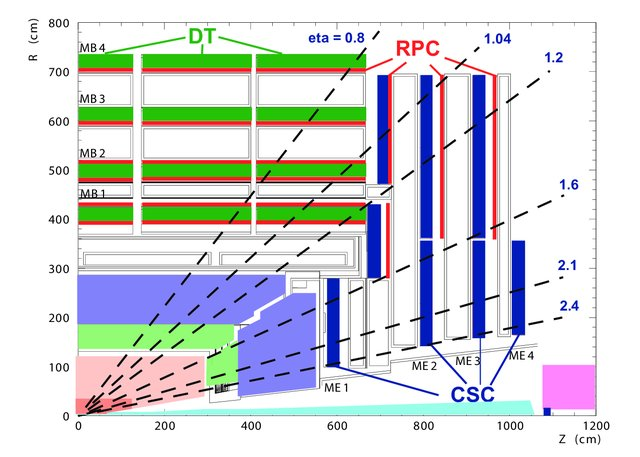
\includegraphics[width=0.98\textwidth,keepaspectratio]{plots_and_figures/chapter3/muon_system_layout.jpg}
\caption{The CMS Muon system layout~\cite{muon1}.}
\label{fig:muon_system_layout}
\end{center}
\end{figure*}

Like all other CMS subdetectors, the muon system is organized into a cylindrical barrel and endcaps. In the barrel region ($|\eta|<1.2)$) the particle rates are low, and magnetic field is uniform~\cite{cms_exp_ref}. This allows for the use DT chambers as detection elements. Each drift tube (42mm by 13 mm, shown in Figure~\ref{fig:drift_tube}) contains a positively charged stretched wire within a gas volume. The gas (85\% Argon (Ar) and 15\% Carbon Dioxide ($\mathrm{CO}_{2}$)) is ionized by muons. Using the positions where the electrons hit on the anode wire and the distance away from the wire (calculated by multiplying the speed of an electron in the tube by the time taken), the coordinates for a muon's position can be calculated. The DT chambers give a position resolution of 100\,$\mu$m, and consist of several groups of alternating layers, with each layercontaining up to 60 DTs.      

\begin{figure*}
\begin{center}
  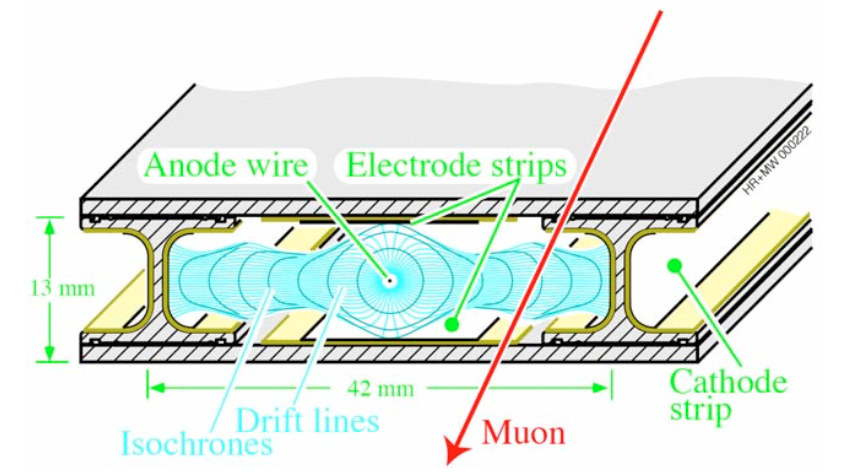
\includegraphics[width=0.75\textwidth,keepaspectratio]{plots_and_figures/chapter3/drift_tube.png}
\caption{A Drift tube schematic~\cite{cms_exp_ref}.}
\label{fig:drift_tube}
\end{center}
\end{figure*}

In the endcap region, particle intensities are high and the magnetic field is non-uniform. This makes DTs unsuitable for endcaps, and CSCs are used instead. Each CSC chamber is trapezoidal in shape (Figure~\ref{fig:csc}) and consists of ``intersecting'' arrays of positively-charged wires and  negatively-charged copper strips. This is housed within a gas volume comprised of 40\% Argon (Ar), 50\% Carbon Dioxide ($\mathrm{CO}_{2}$) and 10\% Tetrafluoroethane. Electrons and ions, produced when passing muons ionize the gas, travel to the anode wires and cathode strips respectively. Charge pulses are produced in both the strips and the wires (perpendicular to strips), providing two coordinates for each muon hit. Unlike DTs, CSCs can support the high particle flux and cope with the large and non-uniform magnetic field in this region.


\begin{figure*}
\begin{center}
  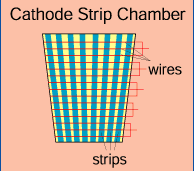
\includegraphics[width=0.6\textwidth,keepaspectratio]{plots_and_figures/chapter3/CSC.png}
\caption{A Cathode Strip Chamber schematic~\cite{muon2}.}
\label{fig:csc}
\end{center}
\end{figure*}

The third component of the muon system are the RPCs which are used specifically for the purpose of triggering on muons, i.e. to make very fast decisions whether or not a muon (having a certain amount of energy or more) is present in the event. Because the response of CSCs and DTs are restricted by their relatively longer drift times, RPCs are placed in both the barrel and endcaps for the purpose of triggering. Just like DTs and CSCs, RPCs are also gas based detectors, consisting of positively-charged anode and negatively-charged cathode plates (made of high resistivity plastic) placed parallel to each other (Figure~\ref{fig:rpc}). The gas that separates these plates (~2.3\,m in length and $\sim$2\,m wide) is composed of 96.2\% Tetrafluoroethane ($\mathrm{C}_{2}\mathrm{H}_{2}\mathrm{F}_{4}$), 3.5\% isobutane ($\mathrm{C}_{2}\mathrm{H}_{10}$) and 0.3\% Sulfur Hexafluoride ($\mathrm{S}\mathrm{F}_{6}$). The fast timing response (1\,ns) of RPCs is achieved by keeping the plates separated by a small consistent distance of about 2\,mm. An avalanche of electrons is produced  when a muon passess through, travels towards the anode plate and is picked up by external metallic strips as a pattern of hits. This gives a quick measure of muon momentum and helps in making fast trigger decisions. Given the bunch crossing time is 25ns, the 1ns timing of RPCs makes them suitable for quickly identifying a muon associated with a particular bunch crossing.      

\begin{figure*}
\begin{center}
  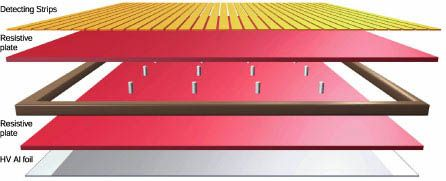
\includegraphics[width=0.6\textwidth,keepaspectratio]{plots_and_figures/chapter3/RPC.jpg}
\caption{A resistive plate chamber schematic~\cite{muon2}.}
\label{fig:rpc}
\end{center}
\end{figure*}

\subsection{The Magnet}
\label{CMS magnet}
The description of the CMS i.e., Compact Muon \textit{Solenoid} is incomplete without a description of its \textit{solenoid} magnet. The CMS magnet is the largest superconducting magnet ever built~\cite{magnet}. It weighs 12,000 tonnes and has an axial magnetic field of 3.8\,T. Like any other solenoid, the CMS magnet is also made of coils of wire that produce a magnetic field when electricity passess through them. The niobium-titanium coils are cooled down to a temperature of $-268.5^{\circ}\,\mathrm{C}$ (a degree higher than outer space) making the magnet superconducting, allowing electricity to flow without resistance and thus producing a very strong magnetic field. The steel yoke of the magnet (within which the muon detectors are interleaved) is responsible for most of the detector's weight, and also provides structural support to the detector. When the magnet is fully powered up it contains about 2.3\,GJ or 638.94\,kWh of energy.

Charged particles trajectories bend in a magnetic field due to the Lorentz force. The stronger the magnetic field is the smaller the radius of curvature of a particle's trajectory is. The more energetic a particle is the larger it its radius of curvature. So, if we know the trajectory of the particle (determined precisely in CMS by the tracker), we can determine its momentum. A strong magnetic field thus necessary for precise measurement of momentum of particles with very high energy.


\subsection{CMS Trigger}
\label{trigger}

The current LHC produces pp collisions at about the rate of 40\,MHz. Considering a typical event size at CMS is~150\,kB, this comes out to be about 5.6 Petabytes per second. Only a small fraction of these events can thus be recorded offline. Even if it were somehow feasible to record this entire volume of data,  most of the collisions produced are mundane soft collisions. We are interested only in events that have certain characteristics, such as events having high transverse momentum of the particles associated with it. The trigger system is used to select these events of interest, making its efficient functioning crucial for physics searches perfomed with the data collected by CMS~\cite{trigger1}. A sophisticated two-level trigger system is thus employed, organized in two consecutive stages- the Level-1 (L1) trigger and the High Level Trigger (HLT).


The L1 trigger is first stage of CMS trigger system. It reduces the rate from 40\,MHz to less than 100\,kHz and has latency of 3.8\,$\mu$s. In other words, it has to make a decision in under 3.8\,$\mu$s. It thus uses only coarse information from the calorimeters and the muon systems, and runs relatively simple algorithms on custom hardware. In particular, it does not use any information from the tracker. The L1 trigger is divided into a L1 Calorimeter Trigger, L1 Muon Trigger, each send information to the Global L1 trigger which makes the decision on wheter to keep or discard the event. The information sent by the L1 Calorimeter Trigger and L1 muon trigger include energy sums (sums of transverse energies deposited on locally grouped sets of crystals, called trigger towers), position, isolation (see section~\ref{isolation}) and quality flags. The global trigger combines this information from the two systems and runs about 300 algorithms in order to make a decision~\cite{trigger2}. The hardware used by the L1 trigger is custom made. Reprogrammble circuits like Field Programmable Gate Arrays (FPGA) form the primary component while application-specific integrated circuits (ASICs) are also used in certain specific use cases.  

Everything that is deemed fit to record by the L1 trigger is received by the HLT. The HLT has relatively longer (~150\,ms) to make a decsision and is fully software-based. It uses information from the entire detector (including the tracker) and partially reconstructs the event. It runs over 400 complex selection algorithms and runs on a massive computer farm. The HLT brings down the output event rate to less than 1 kHz. The events that succesfully pass the HLT selection process are permanently recorded for analysis. 

\subsubsection{Triggers for $\hmue$ and $\Hmue$ searches}
\label{anal_trigger}
For the analyses, only a subset of pp collision data collected by CMS are used. This is chosen by requiring that those events pass (satisfy) a certain trigger depending on the final state signature of the analysis. In the both the analyses, the final state consists of a high $\pt$ muon that comes directly from the Higgs accompanied by a relatively low $\pt$ electron from the tau lepton decay (see sections~\ref{h125_signature} and~\ref{HH_evt_sel}). In $\hmue$ analysis, the data used is composed of events that satisfy a trigger requiring an isolated muon (see section~\ref{isolation}) having a $\pt$ of at least 24\,GeV to be present in the event. In $\Hmue$ analysis, the Higgs Bosons are heavier and $\pt$ requirement is increased to 50\,GeV and there is no isolation requirement on the muon. The same trigger requirement is also required to be passed by simulated samples used in the analysis. The efficiency of the trigger in selecting pp collision events is different to that of its efficiency in selecting simulated samples. This is corrected by using scale factors (depending on $\pt$ and $\eta$) to match the efficiency in simulation to that of the data. The efficiencies were calculated by the CMS Muon Physics Object Group via tag-and-probe methods~\cite{muon_recon2018} using $Z\rightarrow\Pgm\Pgm$ events. Briefly, the tag-and-probe method works in the following way. One of the muons (called the tag) is required to pass strict selection criterion, while the other (called the probe) is required to pass more relaxed criterion. Given the invariant mass of the $\Pgm-\Pgm$ system is required to within a narrow window of the Z mass, the probe muon is also very likely to be a real muon. The percentage of probe muons that pass the criterion we are testing for (identification, isolation, trigger etc.) gives the efficiency. The efficiency plots are shown in Figure~\ref{fig:muon_trigger}.

\begin{figure*}[!htpb]\centering
 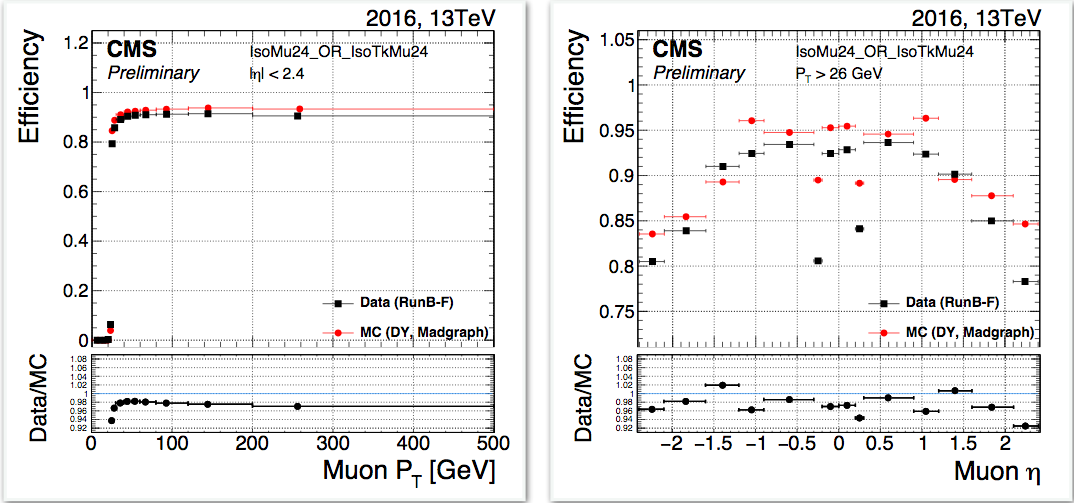
\includegraphics[width=0.9\textwidth,trim=0 -15pt 0 0,clip]{plots_and_figures/chapter3/muontrig1.png}\\
 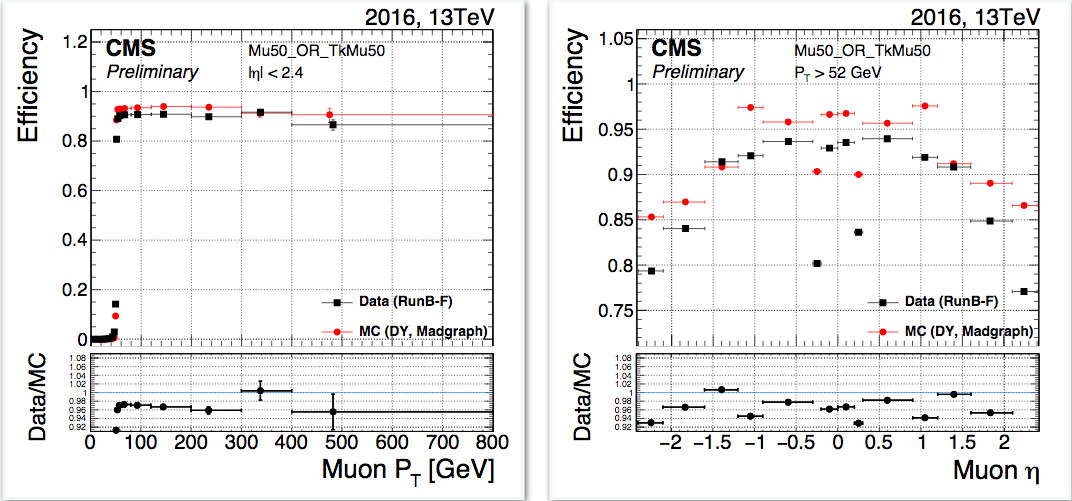
\includegraphics[width=0.9\textwidth]{plots_and_figures/chapter3/muontrig2.png} 
\caption{Efficiency of trigger used in the $\hmue$ analysis (top) and $\Hmue$ analysis (bottom), as a function of $\pt$ (left) and $\eta$ (right), for data (black) and simulation (red).}
 \label{fig:muon_trigger}
\end{figure*}  



